\documentclass{beamer}
%
% Choose how your presentation looks.
%
% For more themes, color themes and font themes, see:
% http://deic.uab.es/~iblanes/beamer_gallery/index_by_theme.html
%
\mode<presentation>
{
  \usetheme{default}      % or try Darmstadt, Madrid, Warsaw, ...
  \usecolortheme{default} % or try albatross, beaver, crane, ...
  \usefonttheme{default}  % or try serif, structurebold, ...
  \setbeamertemplate{navigation symbols}{}
  \setbeamertemplate{caption}[numbered]
} 
\addtobeamertemplate{navigation symbols}{}{%
    \usebeamerfont{footline}%
    \usebeamercolor[fg]{footline}%
    \hspace{1em}%
    \large\insertframenumber/\inserttotalframenumber
}


\renewcommand{\arraystretch}{1.3}
\renewcommand*{\thefootnote}{[\arabic{footnote}]}
%%%%% CHECKS %%%%%

% - font size 20-24

%%%%% CHECKS %%%%%

\usepackage[english]{babel}
\usepackage[utf8x]{inputenc}
\usepackage{amsmath}
\usepackage{siunitx}

\title[Your Short Title]{Measurement of the $2^+_2 \rightarrow 2^+_1$ Electric Monopole Transition Strength in $^{110}$Pd for the Study of Nuclear Structure}
\author{Jonah Berean-Dutcher}
\institute{Department of Physics and Astronomy \newline University of British Columbia}
\footnotetext[1]{TRIUMF}
\begin{document}

%%%%%%%%%%%%%%%%%%%%%%%%%

%%%%%%%%%%%%%%%%%%%%%%%%%

\begin{frame}
  \titlepage
  \begin{block}{Supervisor}
  Reiner Kruecken (TRIUMF)
  \end{block}
\end{frame}

%%%%%%%%%%%%%%%%%%%%%%%%%

%%%%%%%%%%%%%%%%%%%%%%%%%

\begin{frame}{Outline}
 \let\clearpage\relax
 \tableofcontents
\end{frame}



\section{Background}

%%%%%%%%%%%%%%%%%%%%%%%%%

%%%%%%%%%%%%%%%%%%%%%%%%%

\begin{frame}{Background}
\framesubtitle{Shell Model of the Nucleus}
\begin{figure}[!hht]
  \centering
  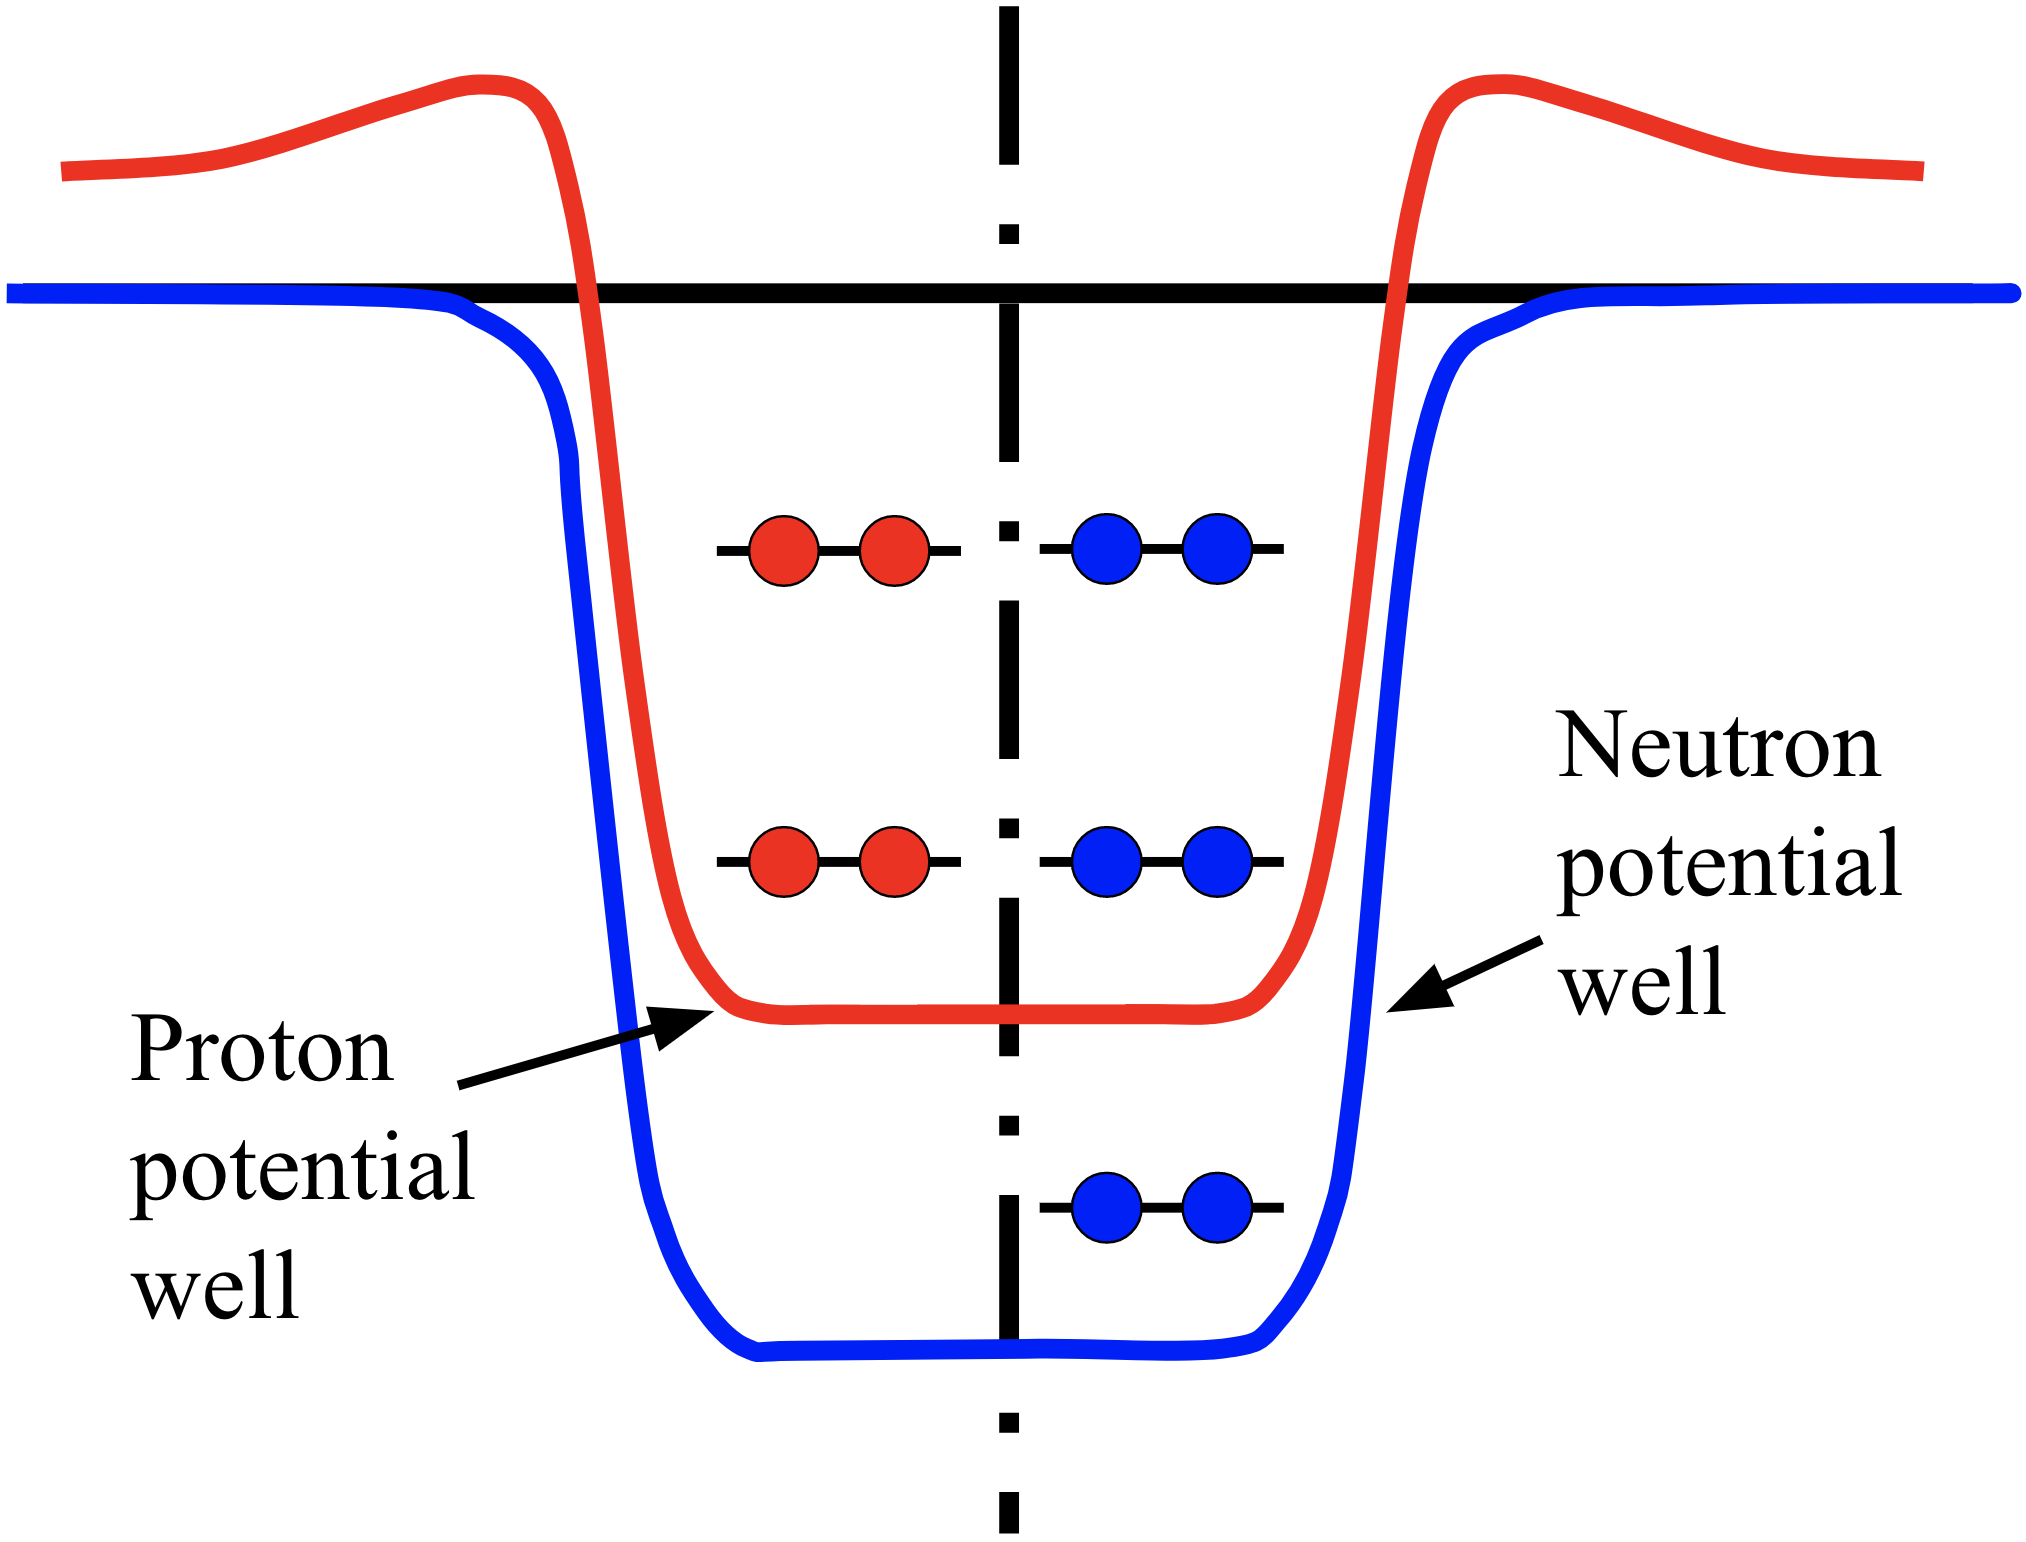
\includegraphics[width=0.85\textwidth, keepaspectratio]{FermiFinal.png}
  \caption{Simple picture of nuclear potentials, and Fermi-gas structure.}
  \label{ShellFermi}
\end{figure}
\end{frame}

%%%%%%%%%%%%%%%%%%%%%%%%%

%%%%%%%%%%%%%%%%%%%%%%%%%

\begin{frame}{Background}
\framesubtitle{Nuclear Landscape}
\begin{figure}[!hht]
  \centering
  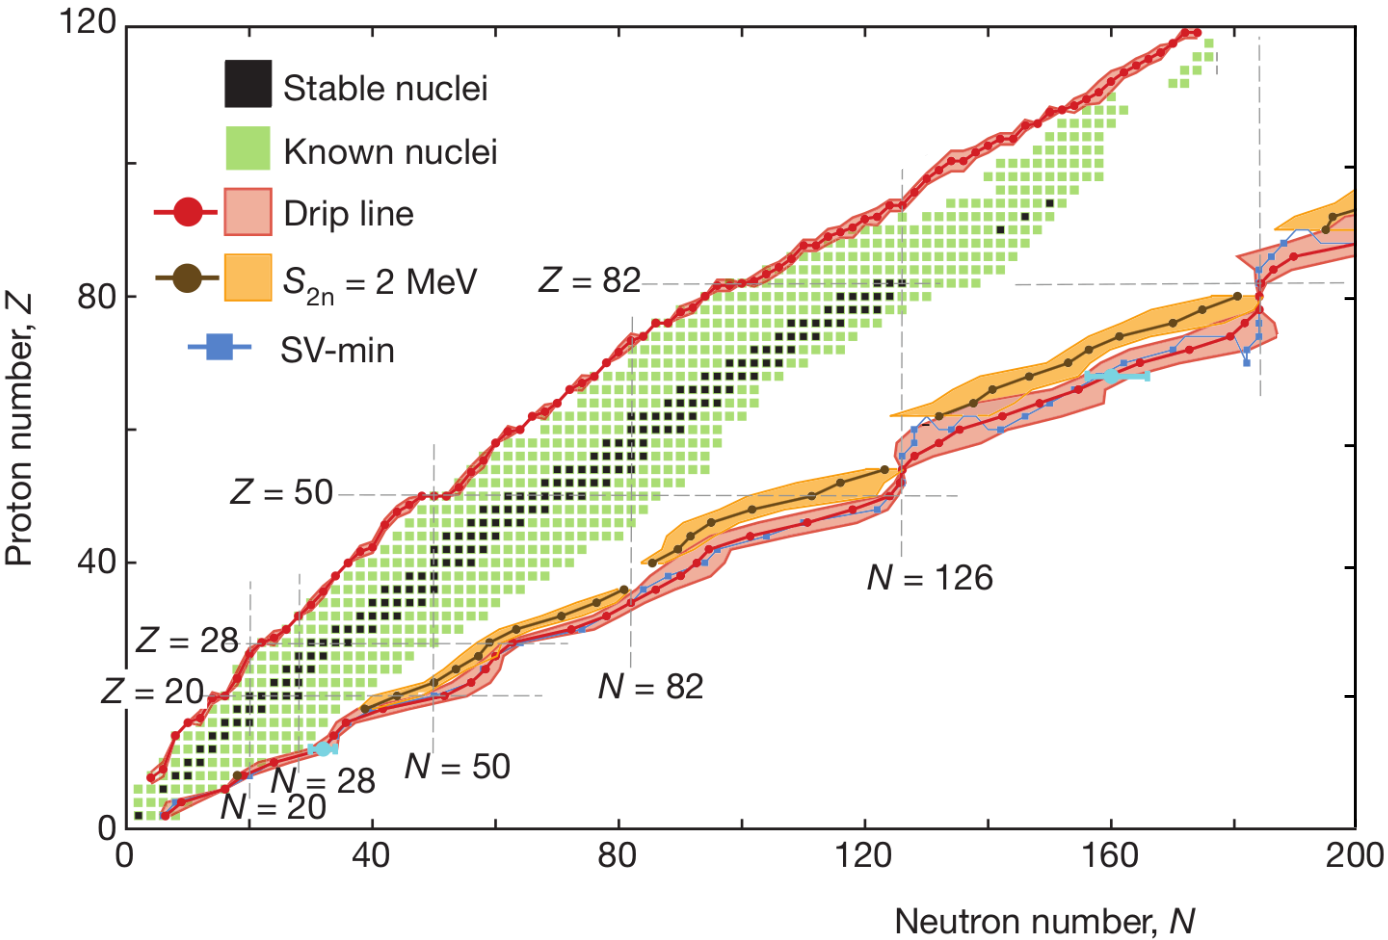
\includegraphics[width=0.85\textwidth, keepaspectratio]{NuclearLimit.png}
  \caption{The nuclear chart with theoretically predicted limits\footnotemark[1].}
  \label{ShellFermi}
\end{figure}
\footnotetext[1]{\tiny{J.~Erler et. al. \textit{The chart of known nuclei. The limits of existence for the chart are predicted from nuclear theory.} Nature 486, 509–512 (2012)}}
\end{frame}

%%%%%%%%%%%%%%%%%%%%%%%%%

%%%%%%%%%%%%%%%%%%%%%%%%%

\begin{frame}{Background}
\framesubtitle{Nuclear Deformation as a Collective Response to Energy Potential}
\begin{figure}[!hht]
  \centering
  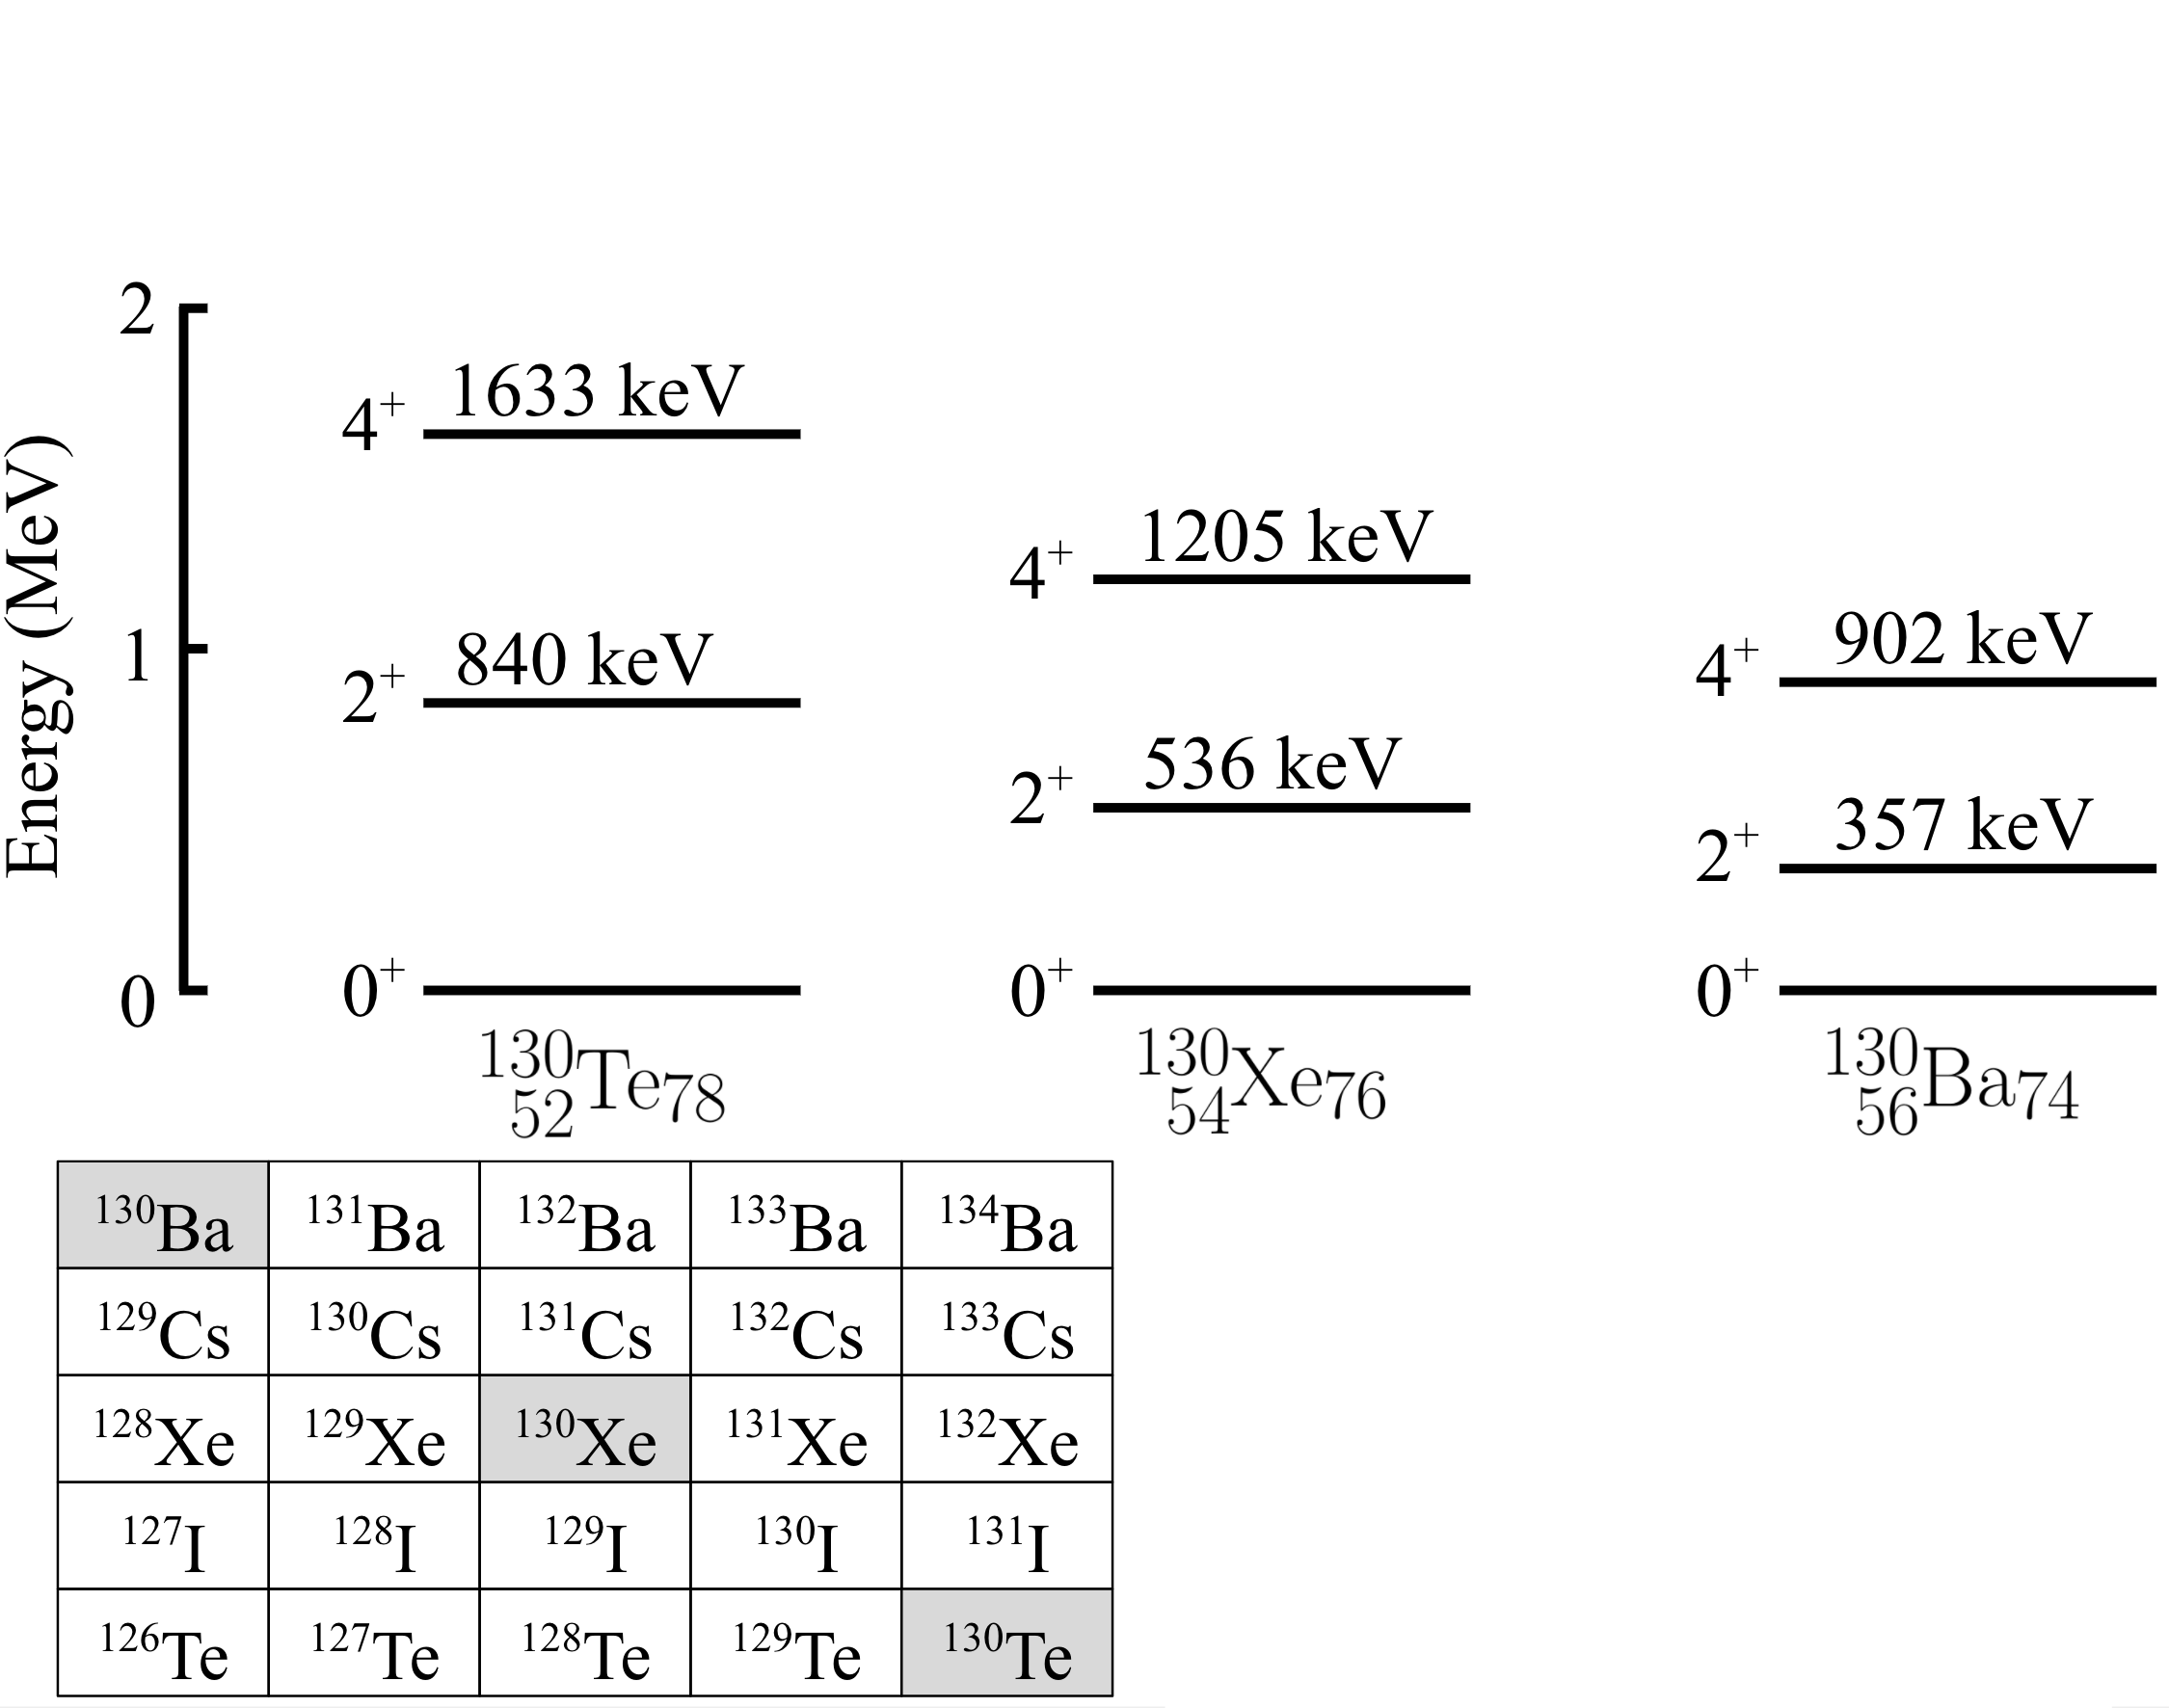
\includegraphics[width=0.9\textwidth, keepaspectratio]{CastenLevels_1.png}
\end{figure}
\end{frame}

\begin{frame}{Background}
\framesubtitle{Nuclear Deformation as a Collective Response to Energy Potential}
\begin{figure}[!hht]
  \centering
  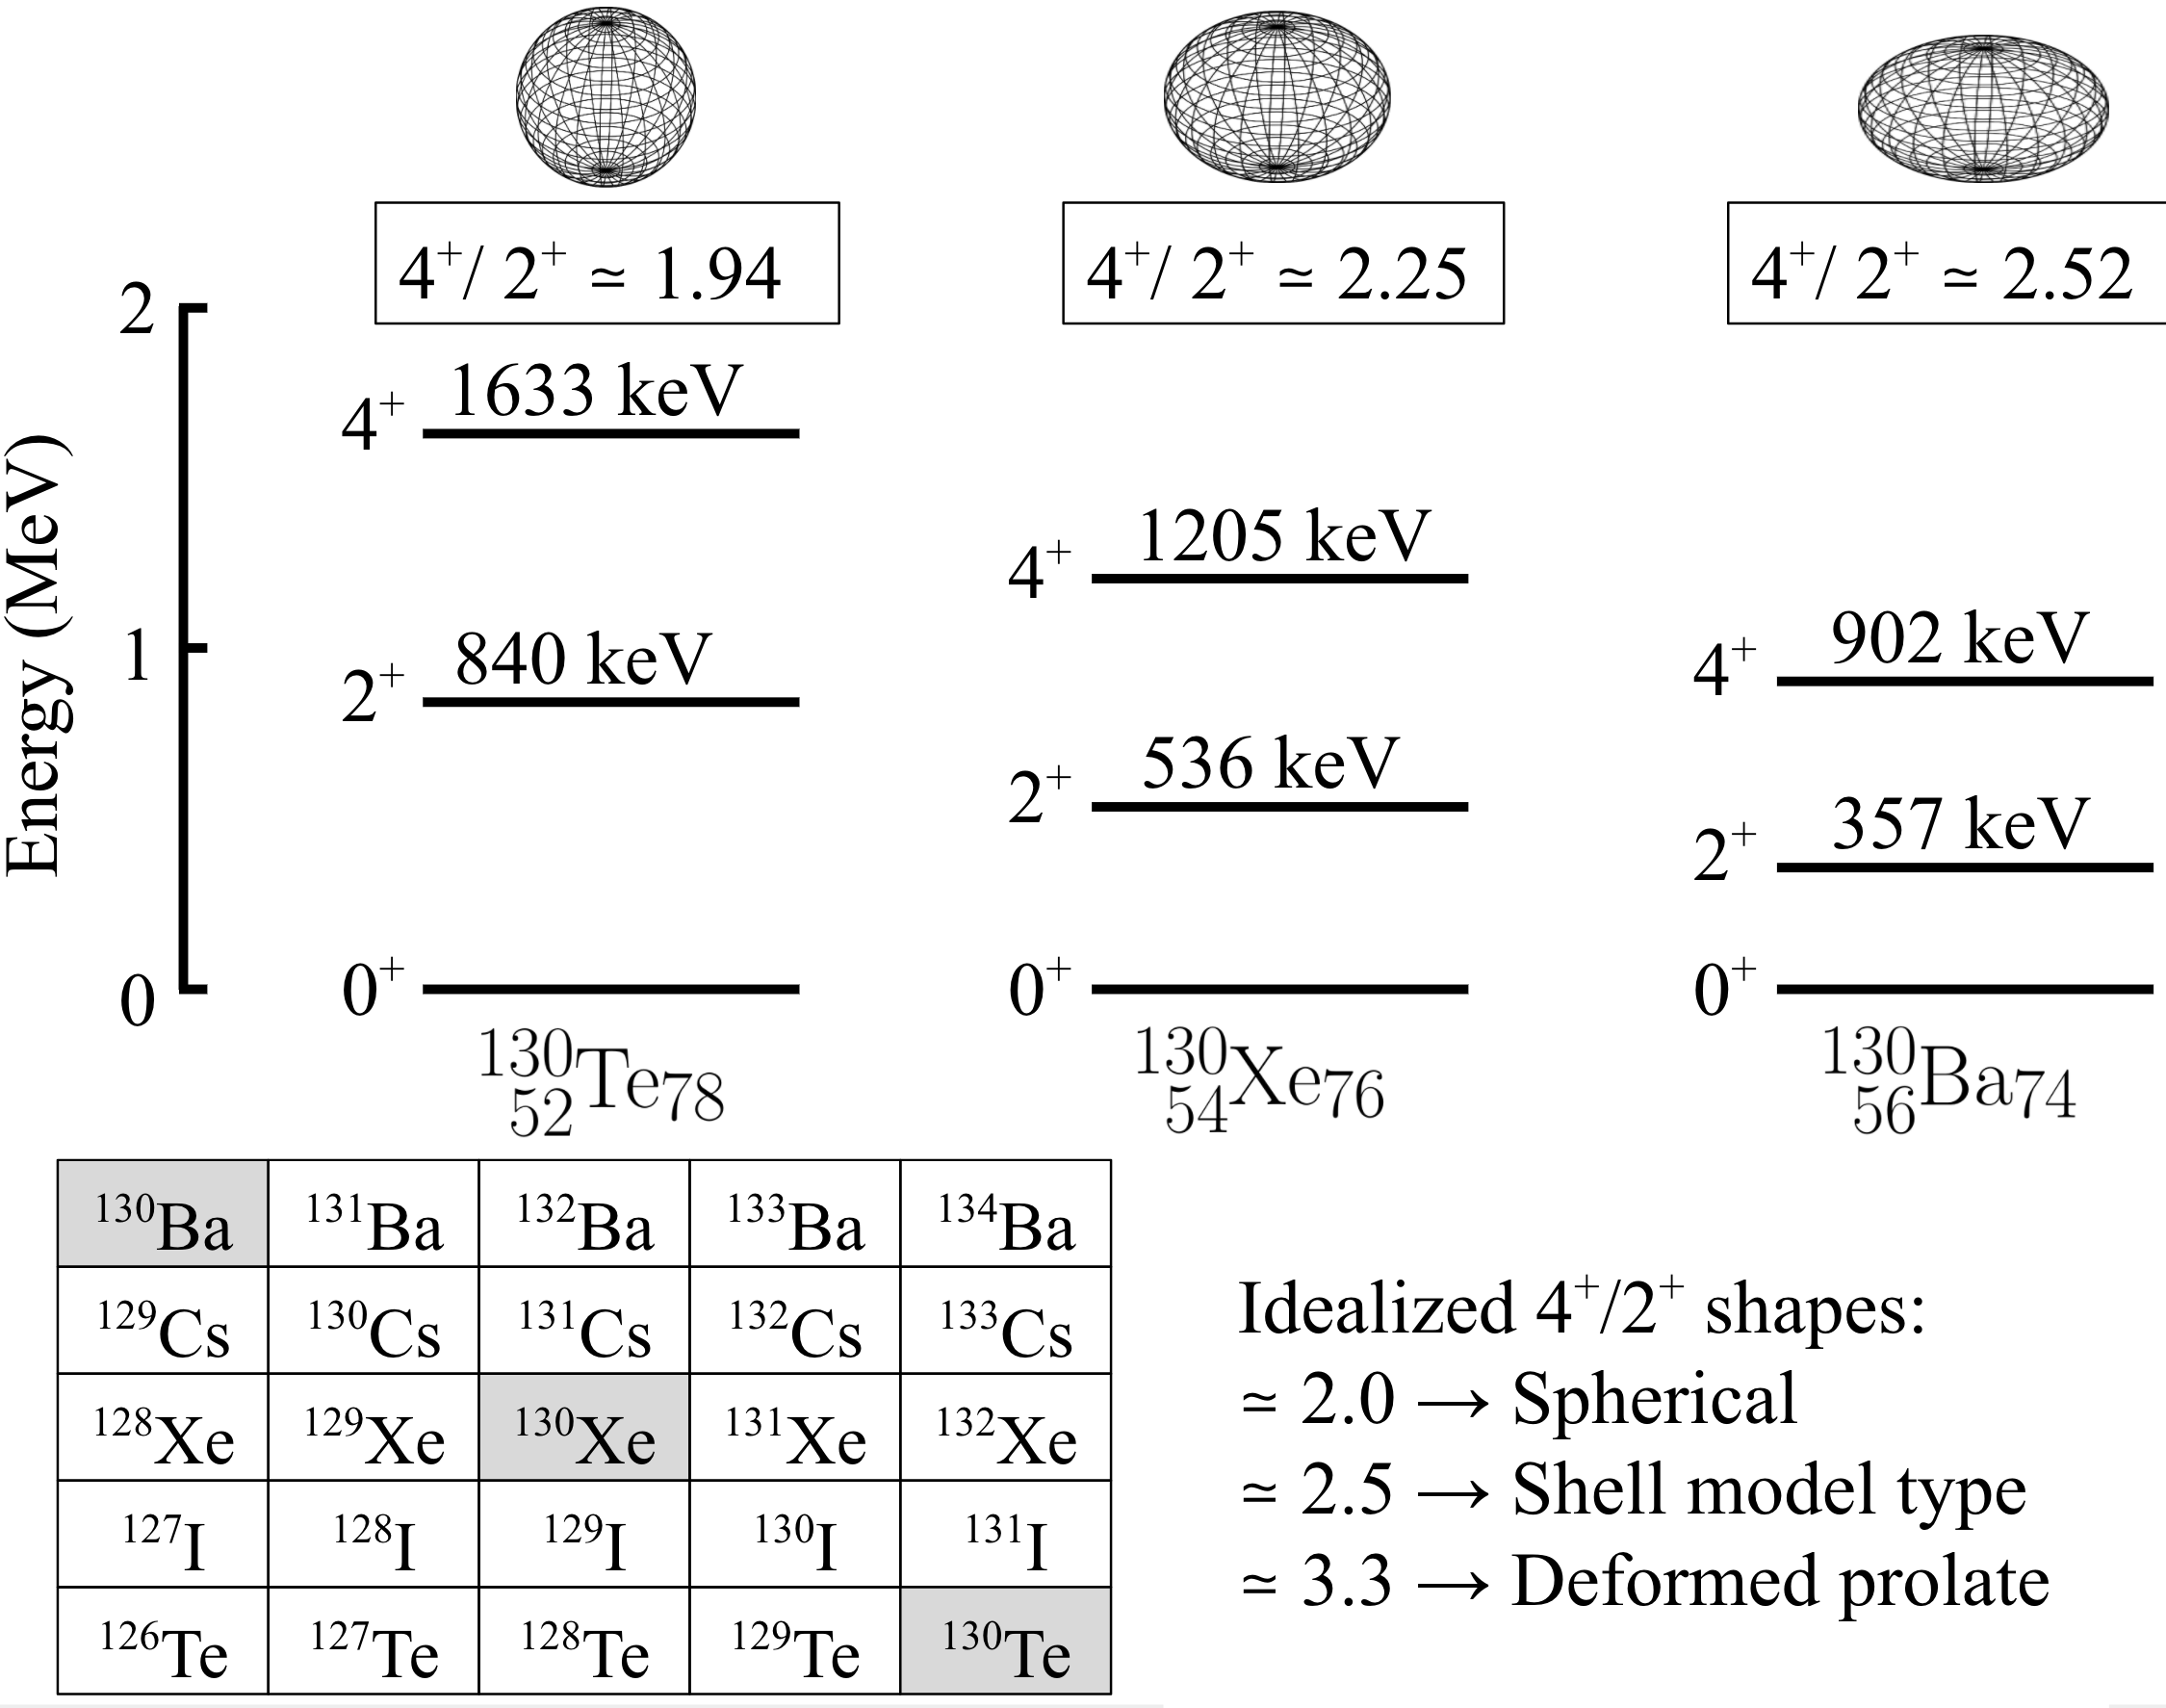
\includegraphics[width=0.9\textwidth, keepaspectratio]{CastenLevels_2.png}
\end{figure}
\end{frame}

%%%%%%%%%%%%%%%%%%%%%%%%%

%%%%%%%%%%%%%%%%%%%%%%%%%

\begin{frame}{Background}
\framesubtitle{Nuclear Shape Across the Chart}
\begin{figure}[!hht]
  \centering
  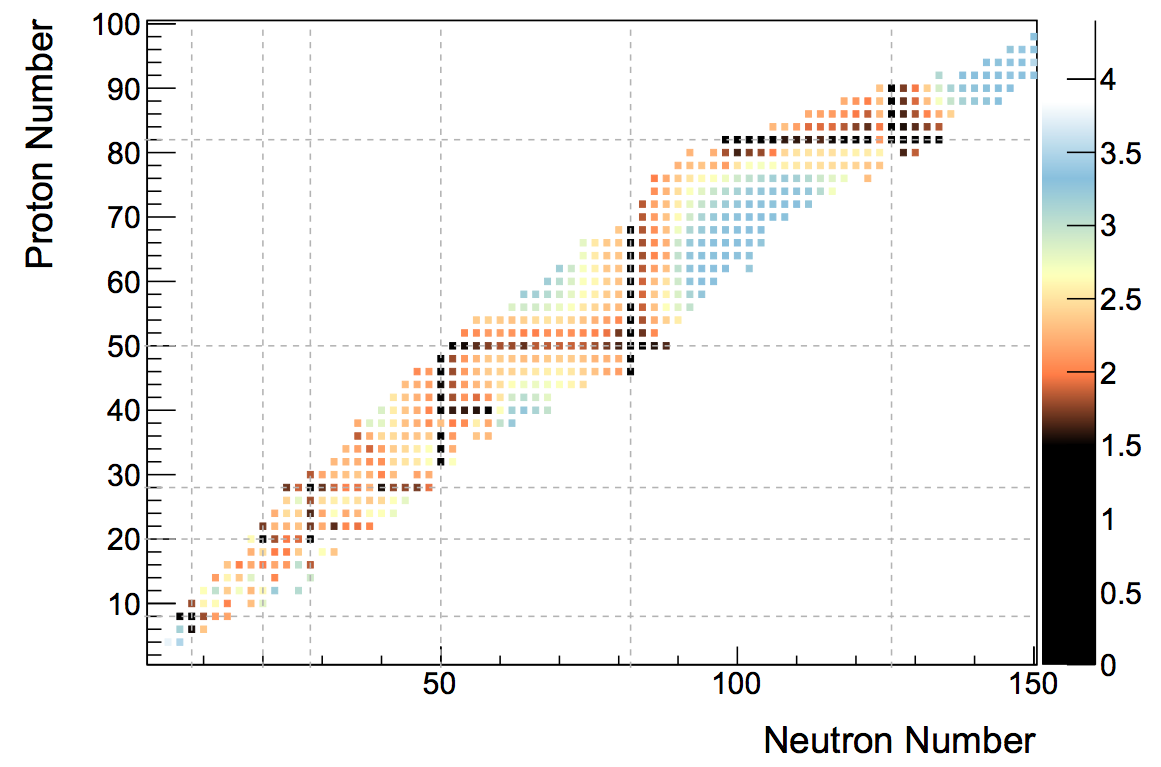
\includegraphics[width=0.85\textwidth, keepaspectratio]{Evitts4and2.png}
  \caption{The ratio of $4^+_1$ to $2^+_1$ empirical energies for each nuclide across the chart\footnotemark[1].}
  \label{comparison}
\end{figure}
\footnotetext[1]{\tiny{L. J. Evitts. \textit{PENS: Parsing ENSDF.} https://doi.org/10.5281/zenodo.376872, March 2017.}}
\end{frame}

%%%%%%%%%%%%%%%%%%%%%%%%%

%%%%%%%%%%%%%%%%%%%%%%%%%

\begin{frame}{Background}
\framesubtitle{Shape Coexistence and Mixing}
\begin{figure}[!hht]
  \centering
  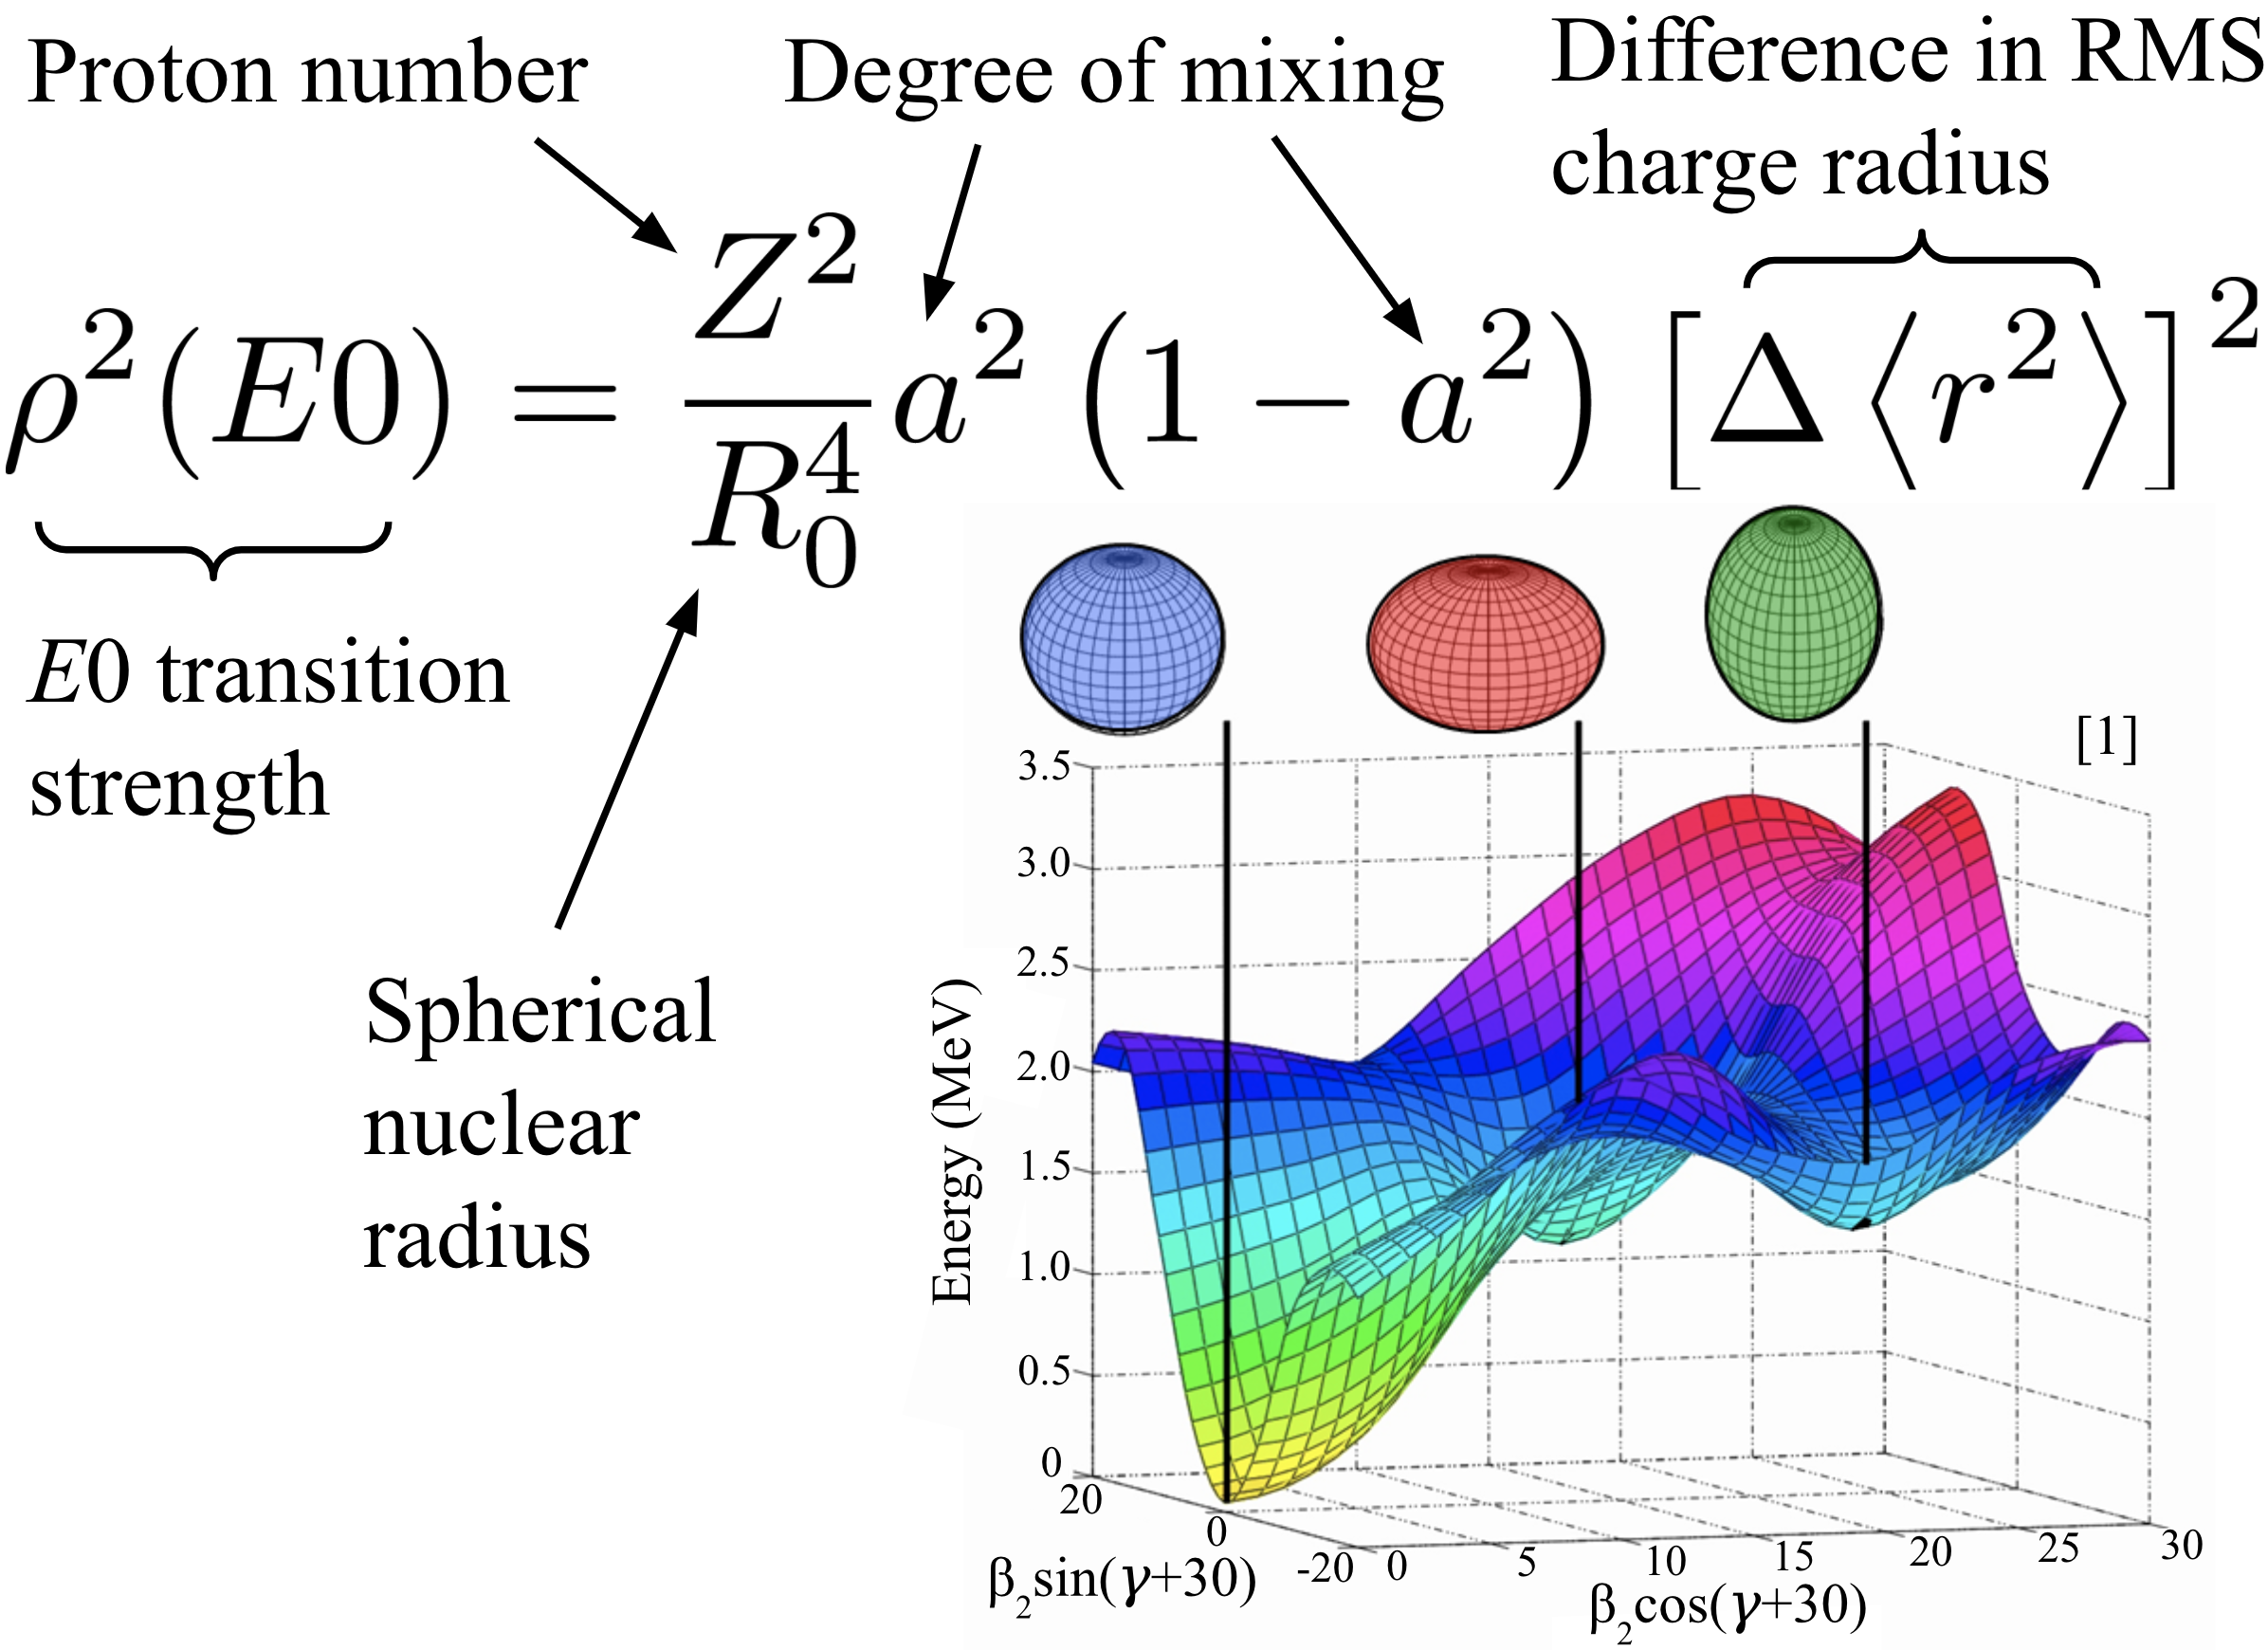
\includegraphics[width=0.8\textwidth, keepaspectratio]{ShapeCoexistenceAndMixing.png}
  \label{geopE0}
\end{figure}
\footnotetext[1]{A Andreyev et al. \textit{A triplet of differently shaped spin-zero states in the atomic nucleus $^{186}\mathrm{Pb}$.} Nature 405, 430 (2000)}
\end{frame}

%%%%%%%%%%%%%%%%%%%%%%%%%

%%%%%%%%%%%%%%%%%%%%%%%%%

\begin{frame}{Background}
\framesubtitle{Measured $B(E2)$}
\begin{figure}[!hht]
  \centering
  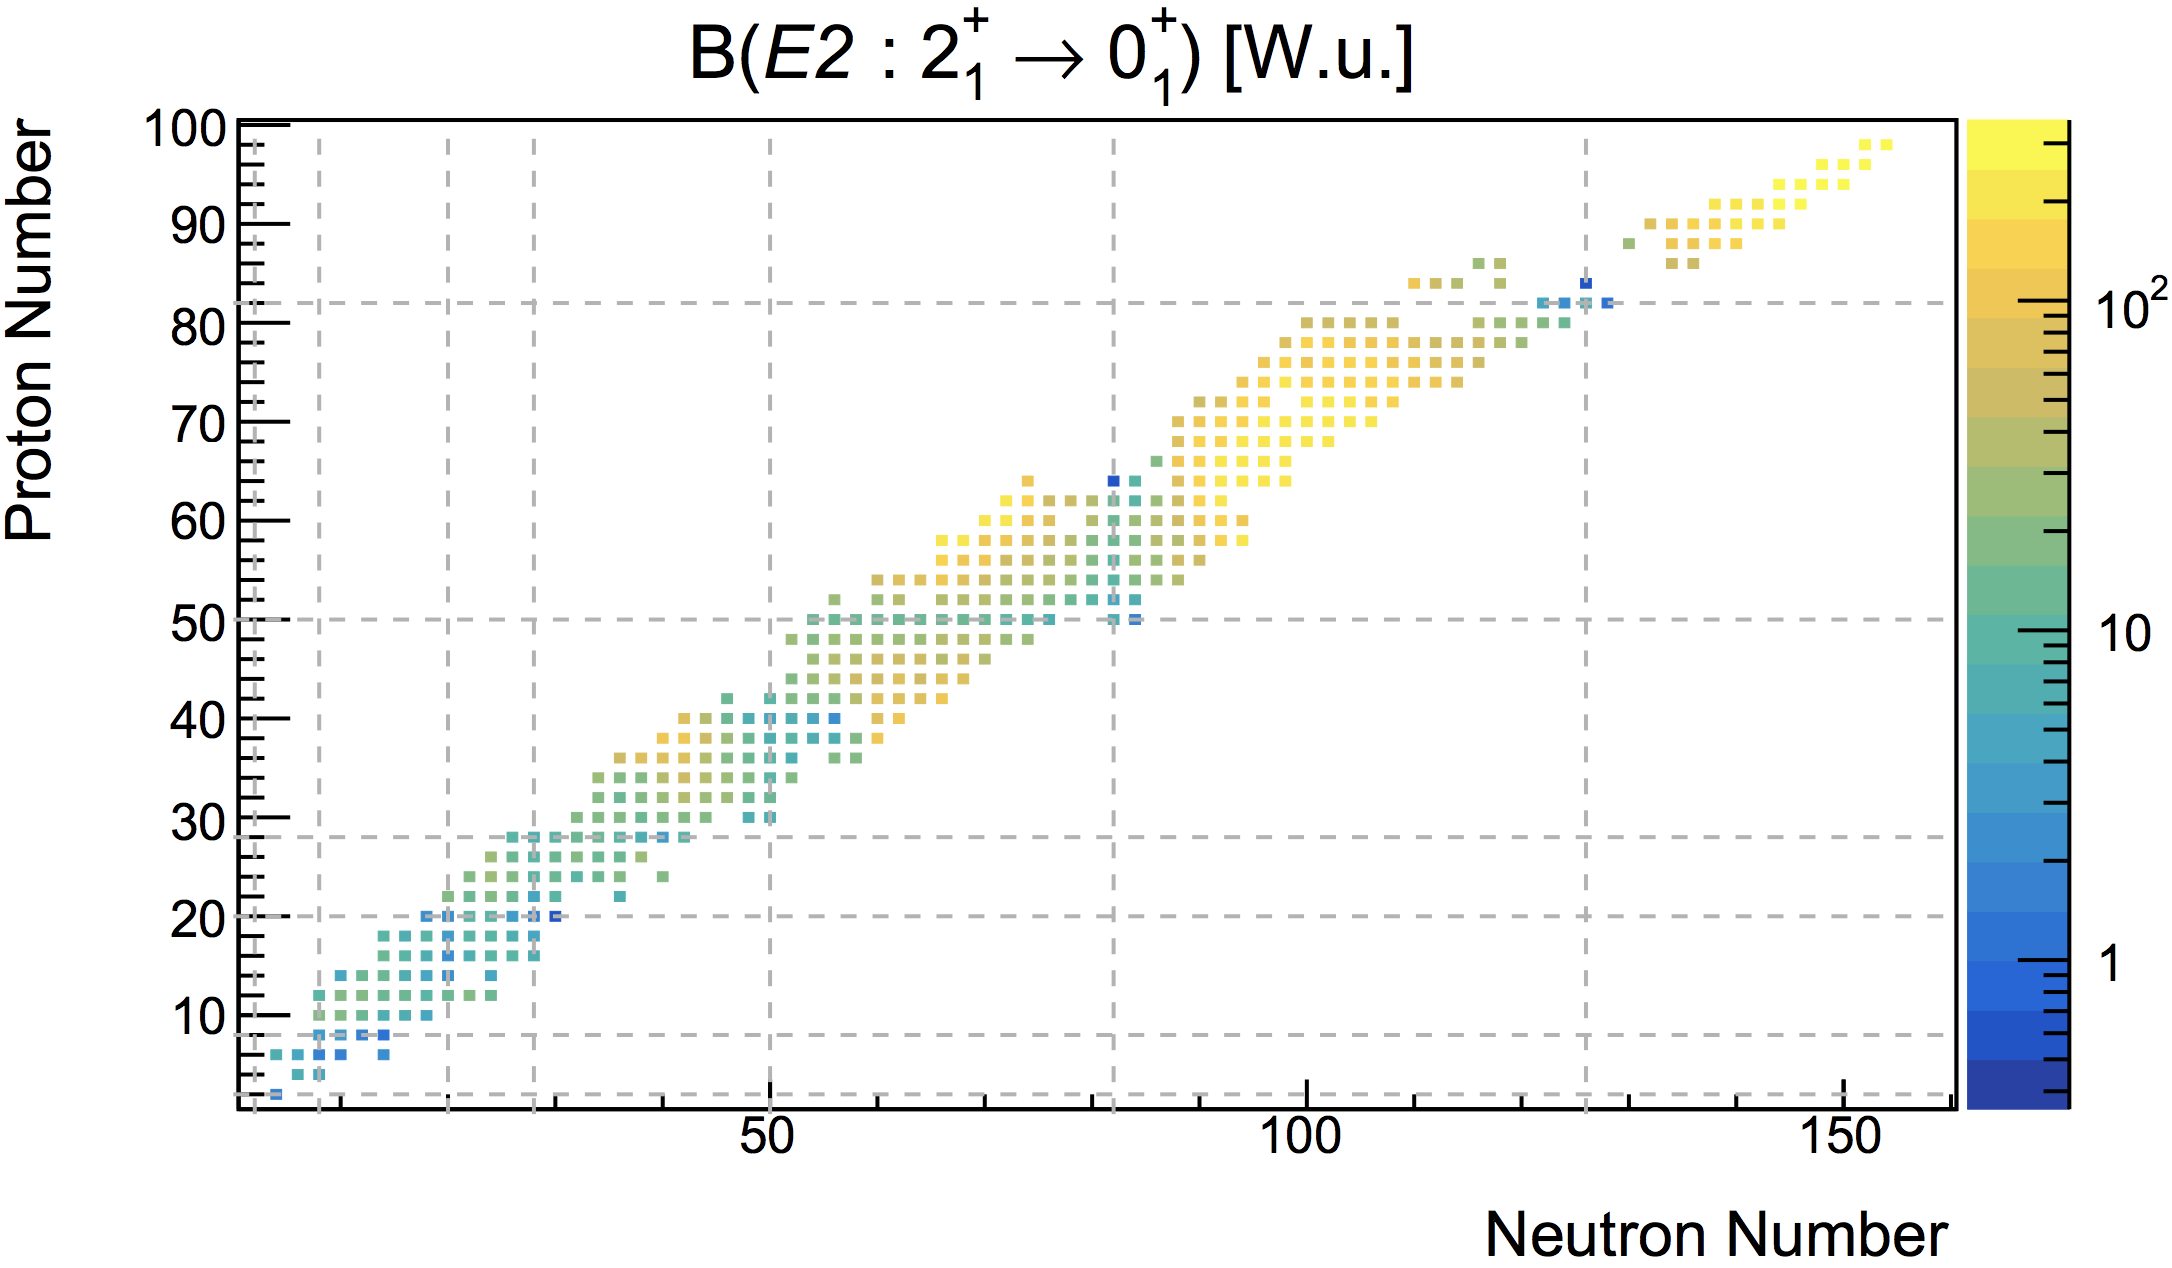
\includegraphics[width=0.95\textwidth, keepaspectratio]{EvittsE2.png}
  \caption{The known $B(E2)$ values (399 total) between the first $2^+$ and ground state\footnotemark[1].}
  \label{comparisonE2}
\end{figure}
\footnotetext[1]{B. Pritychenko et al. Atomic Data and Nuclear Tables, 107:1 - 139, 2016.}
\end{frame}

%%%%%%%%%%%%%%%%%%%%%%%%%

%%%%%%%%%%%%%%%%%%%%%%%%%

\begin{frame}{Background}
\framesubtitle{Measured $\rho^2(E0)$; $0_2^+ \rightarrow 0_1^+$}
\begin{figure}[!hht]
  \centering
  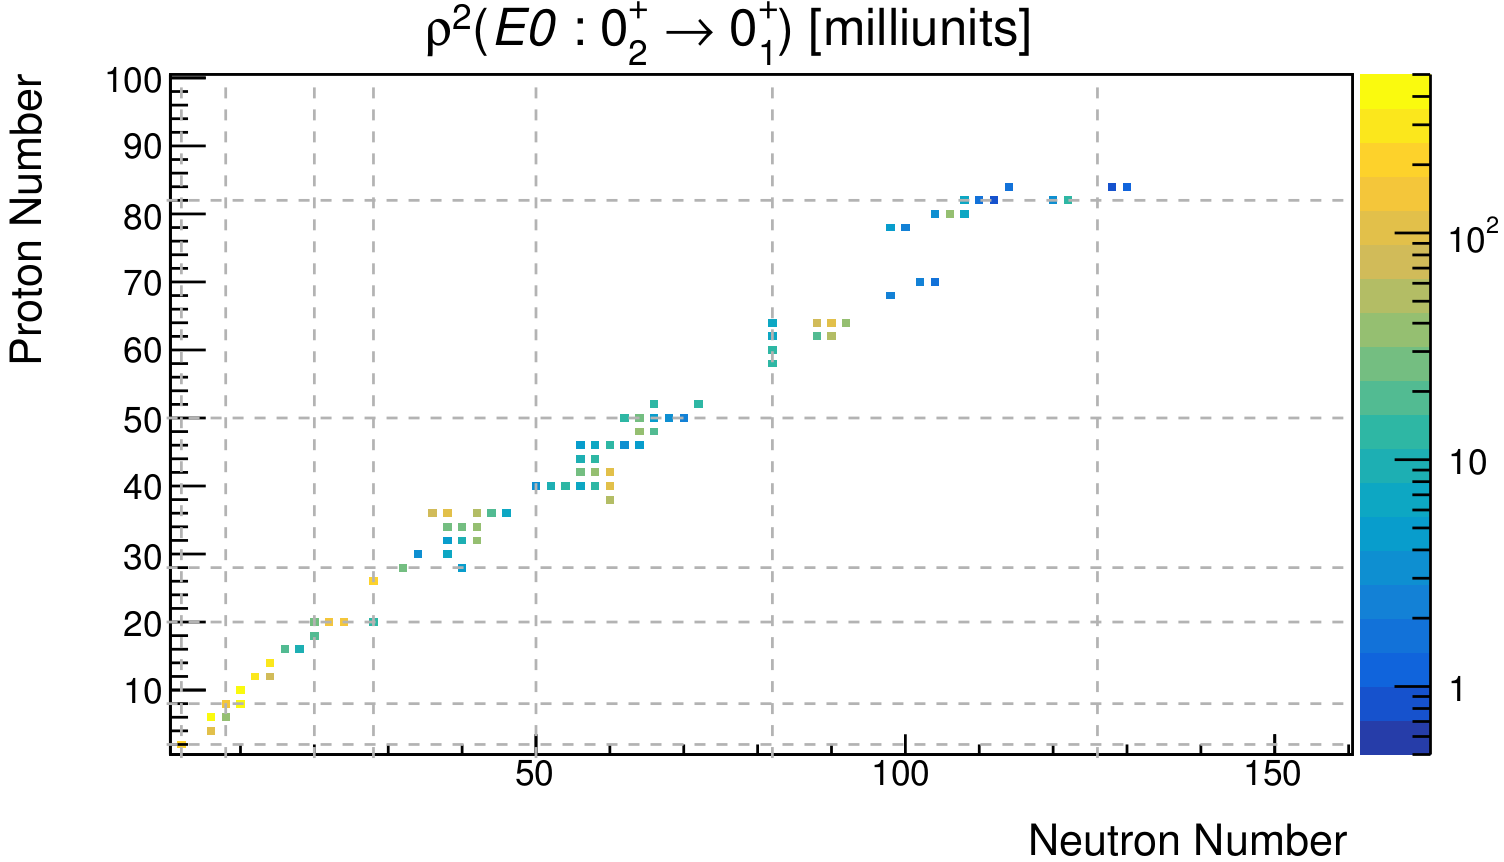
\includegraphics[width=0.95\textwidth, keepaspectratio]{0to0Chart.png}
  \caption{The known $\rho^2(E0)$ values (84 total) for the second $0^+$ to the ground state.\footnotemark[1]}
  \label{comparisonE0for0}
\end{figure}
\footnotetext[1]{Kibedi et al. Atomic and Nuclear Data Tables, 89(1):77-100, 2005.}
\end{frame}

%%%%%%%%%%%%%%%%%%%%%%%%%

%%%%%%%%%%%%%%%%%%%%%%%%%

\begin{frame}{Background}
\framesubtitle{Measured $\rho^2(E0)$; $2_2^+ \rightarrow 2_1^+$}
\begin{figure}[!hht]
  \centering
  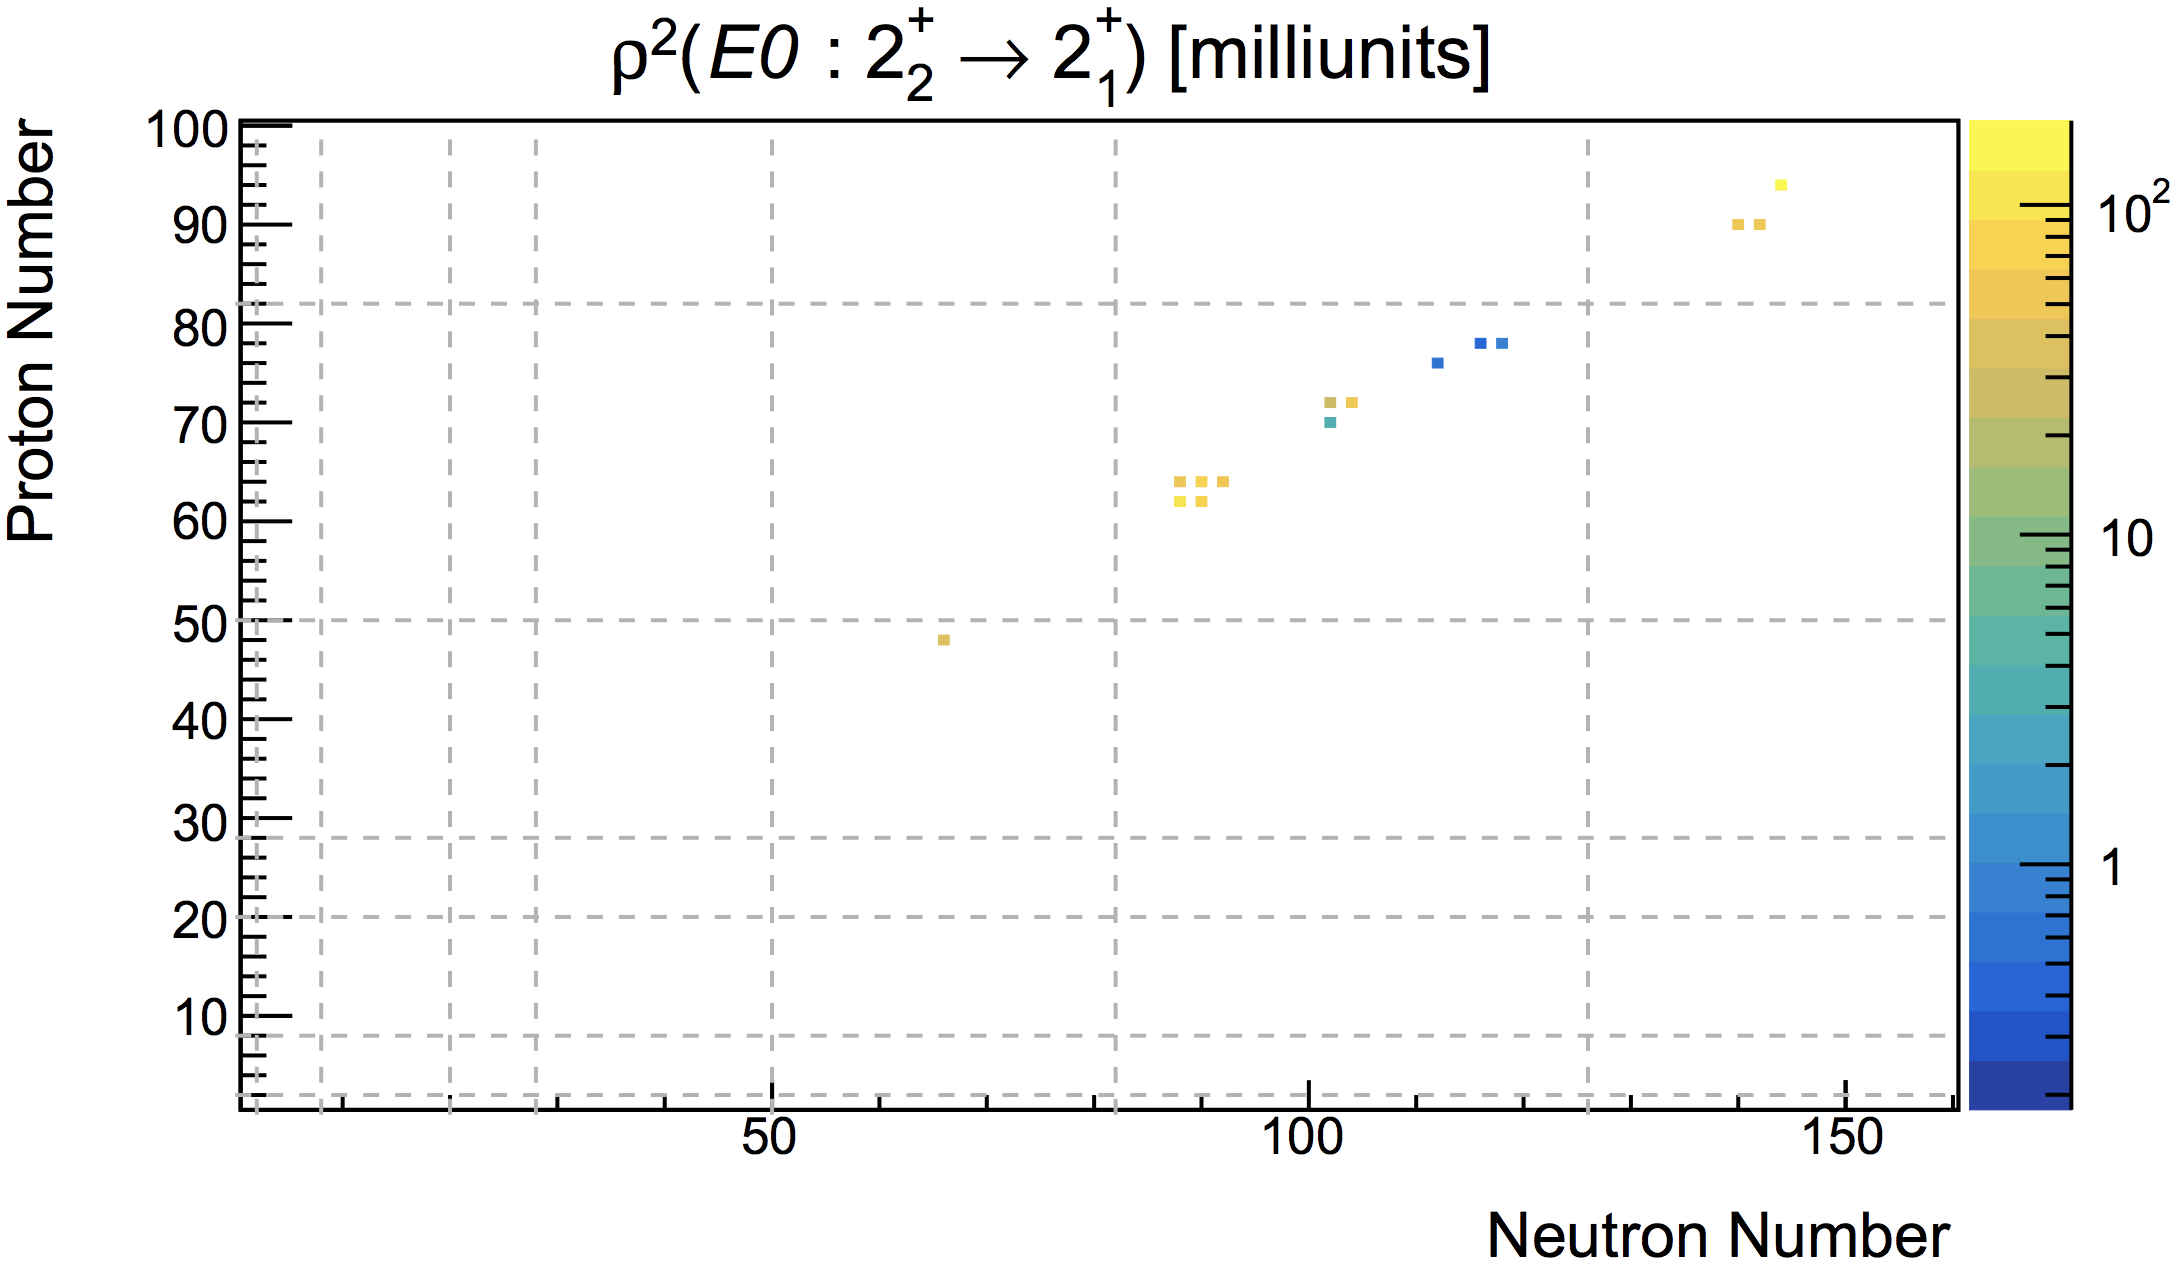
\includegraphics[width=0.95\textwidth, keepaspectratio]{EvittsE0.png}
  \caption{The known $\rho^2(E0)$ values (15 total) for the second excited $2^+$ to the first excited $2^+$ state\footnotemark[1].}
  \label{comparisonE0for2}
\end{figure}
\footnotetext[1]{Wood et al. Nuclear Physics A 651 (1999) 323-368.}
\end{frame}

%%%%%%%%%%%%%%%%%%%%%%%%%

%%%%%%%%%%%%%%%%%%%%%%%%%

\section{Methods: $\gamma$-ray and $e^-$ Spectroscopy}

% \begin{frame}{Methods}
% \framesubtitle{Experiment: Alpha Scattering Above the Coulomb Barrier}
% \begin{figure}[!ht]
%   \centering
%   \includegraphics[width=0.8\textwidth,keepaspectratio]{ExpSchematic.png}
%   \caption{Diagram showing the setup for the experiment, with an alpha nucleus scattering off a $^{110}\mathrm{Pd}$ target nucleus into the S3 detector; emitting electrons and $\gamma$ rays.}
%   \label{diagram}
% \end{figure} 
% \end{frame}

%%%%%%%%%%%%%%%%%%%%%%%%%

%%%%%%%%%%%%%%%%%%%%%%%%%

\begin{frame}{Methods}
\framesubtitle{SPICE and TIGRESS}
\begin{figure}[!hht]
  \centering
  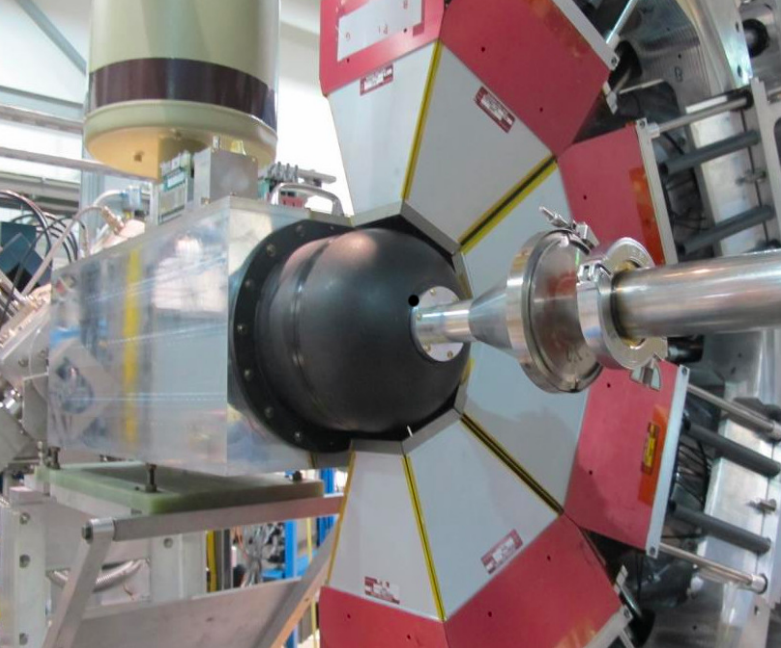
\includegraphics[width=0.46\textwidth, keepaspectratio]{SPICE.png}
  \hspace{0.3cm}
  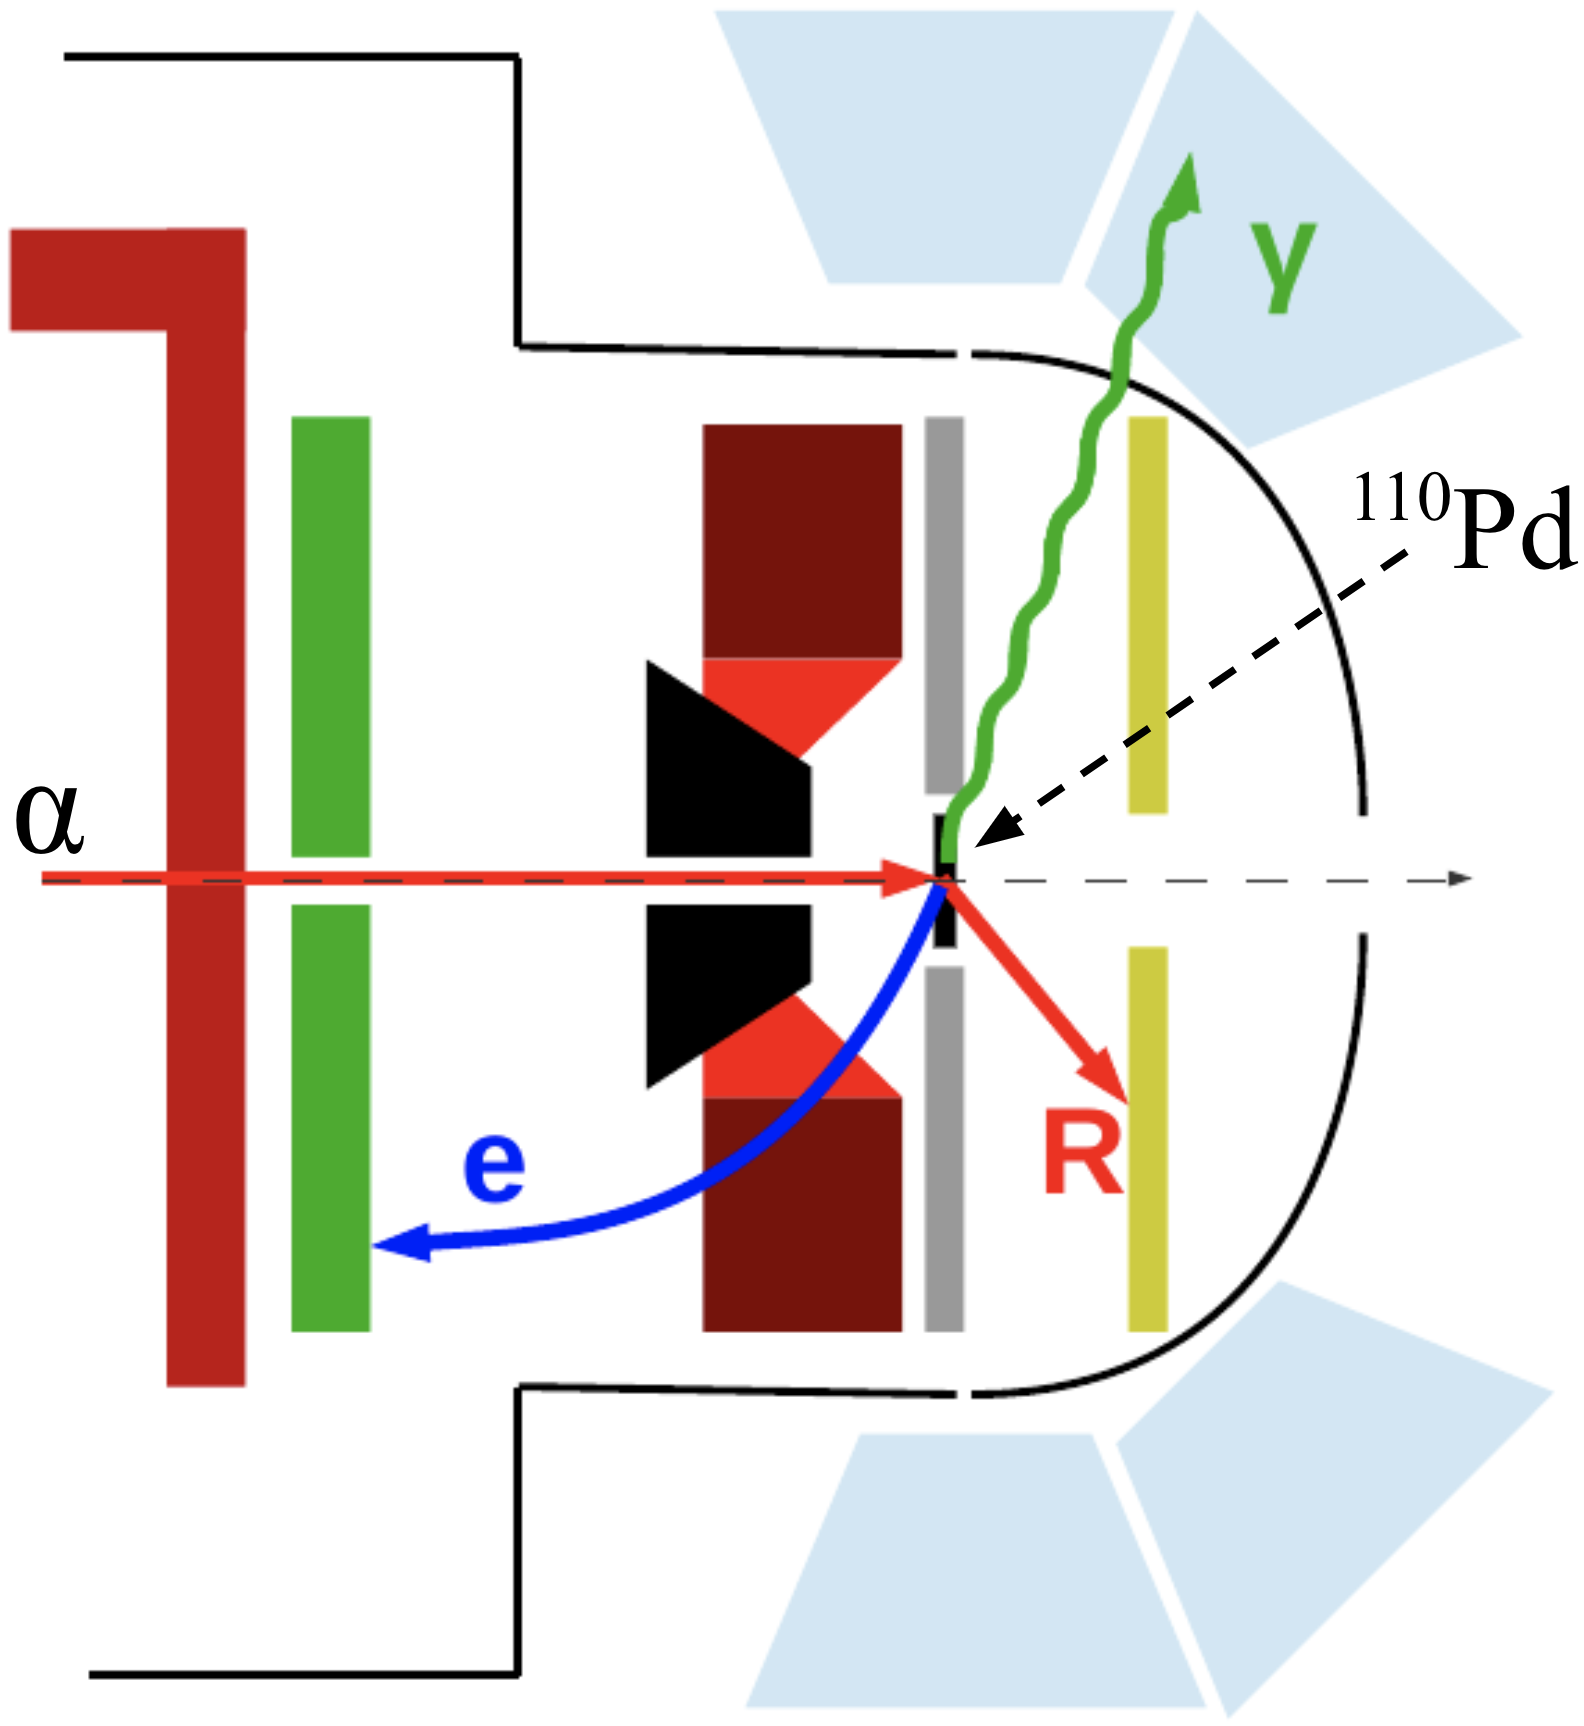
\includegraphics[width=0.46\textwidth, keepaspectratio]{SPICESchem.png}
  \caption{Photo, Schematic of SPICE (Spectrometer for Internal Conversion Electrons) and
TIGRESS (TRIUMF-ISAC Gamma-Ray Escape Suppressed Spectrometer)}
\end{figure}
\end{frame}

%%%%%%%%%%%%%%%%%%%%%%%%%

%%%%%%%%%%%%%%%%%%%%%%%%%

% \begin{frame}{Methods}
% \framesubtitle{SPICE and TIGRESS}
% \begin{figure}[!hht]
%   \centering
%   \includegraphics[width=0.6\textwidth, keepaspectratio]{Full.png}
% \end{figure}
% \end{frame}

%%%%%%%%%%%%%%%%%%%%%%%%%

%%%%%%%%%%%%%%%%%%%%%%%%%

\begin{frame}{Methods}
\framesubtitle{The Nucleus $^{110}\mathrm{Pd}$}
\begin{figure}[!hht]
  \centering
  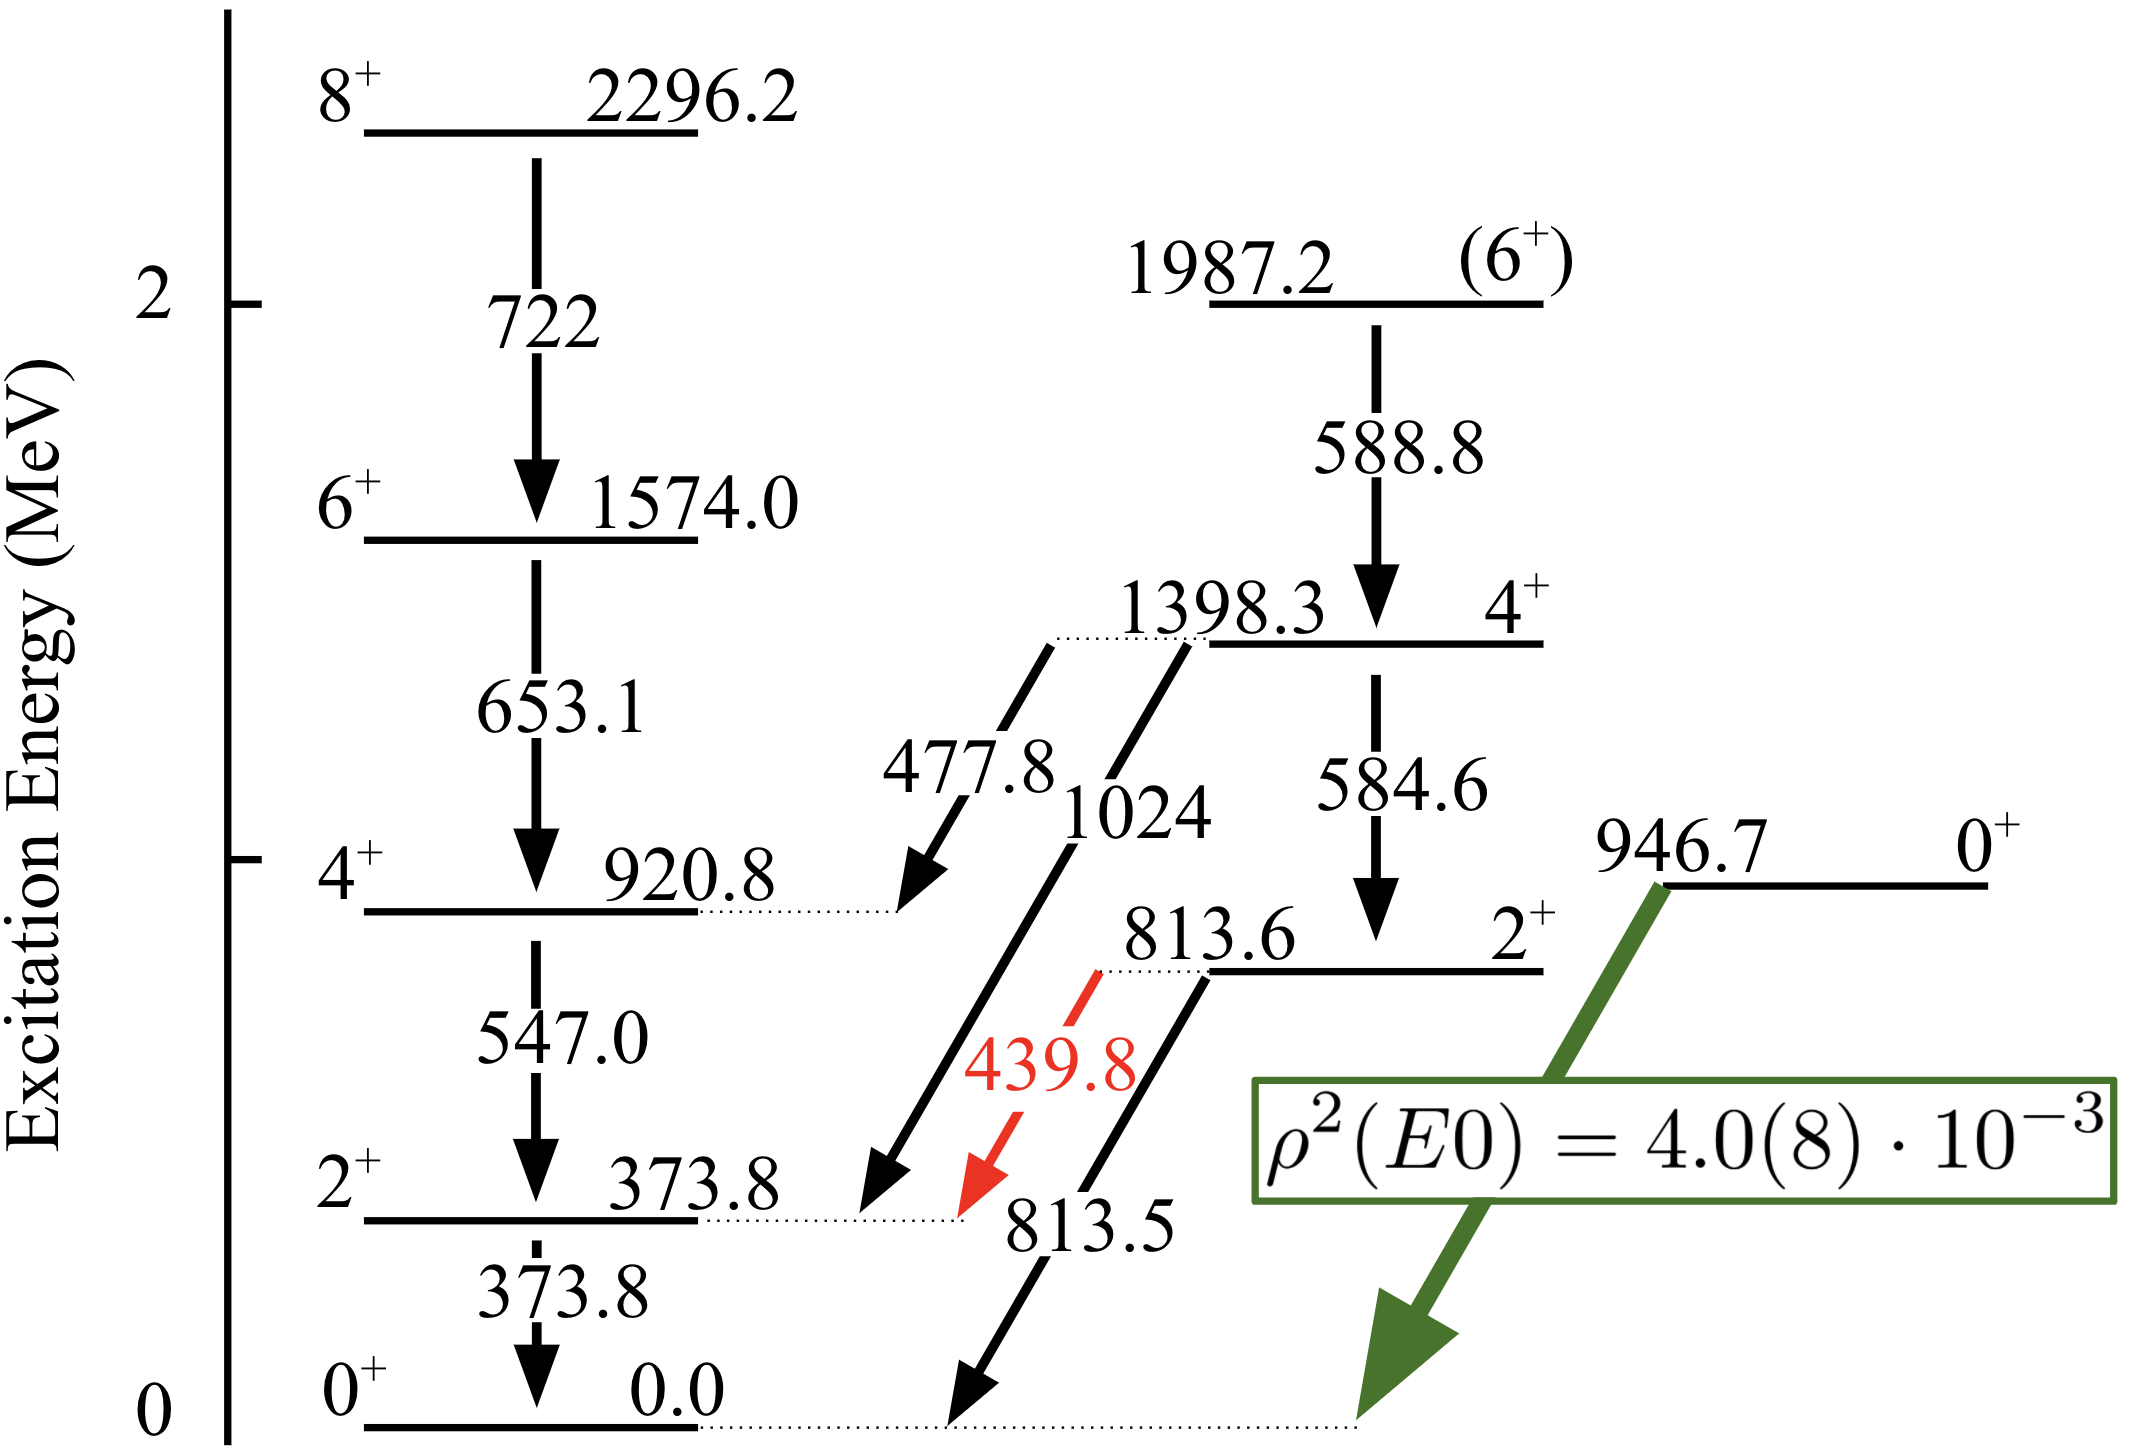
\includegraphics[width=0.8\textwidth, keepaspectratio]{110PdLevels.png}
  \caption{Partial level scheme for $^{110}\mathrm{Pd}$\footnotemark[1].}
  \label{comparison}
\end{figure}
\footnotetext[1]{G. G$\ddot{u}$rdal and F. G. Kondev, \textit{Evaluated nuclear structure data file}, NDS 113, 1315 (2012).}
\end{frame}

\begin{frame}{Methods}
\framesubtitle{$E0$ Transitions Forbidden for $\Delta K \neq 0$}
\begin{figure}[!hht]
  \centering
  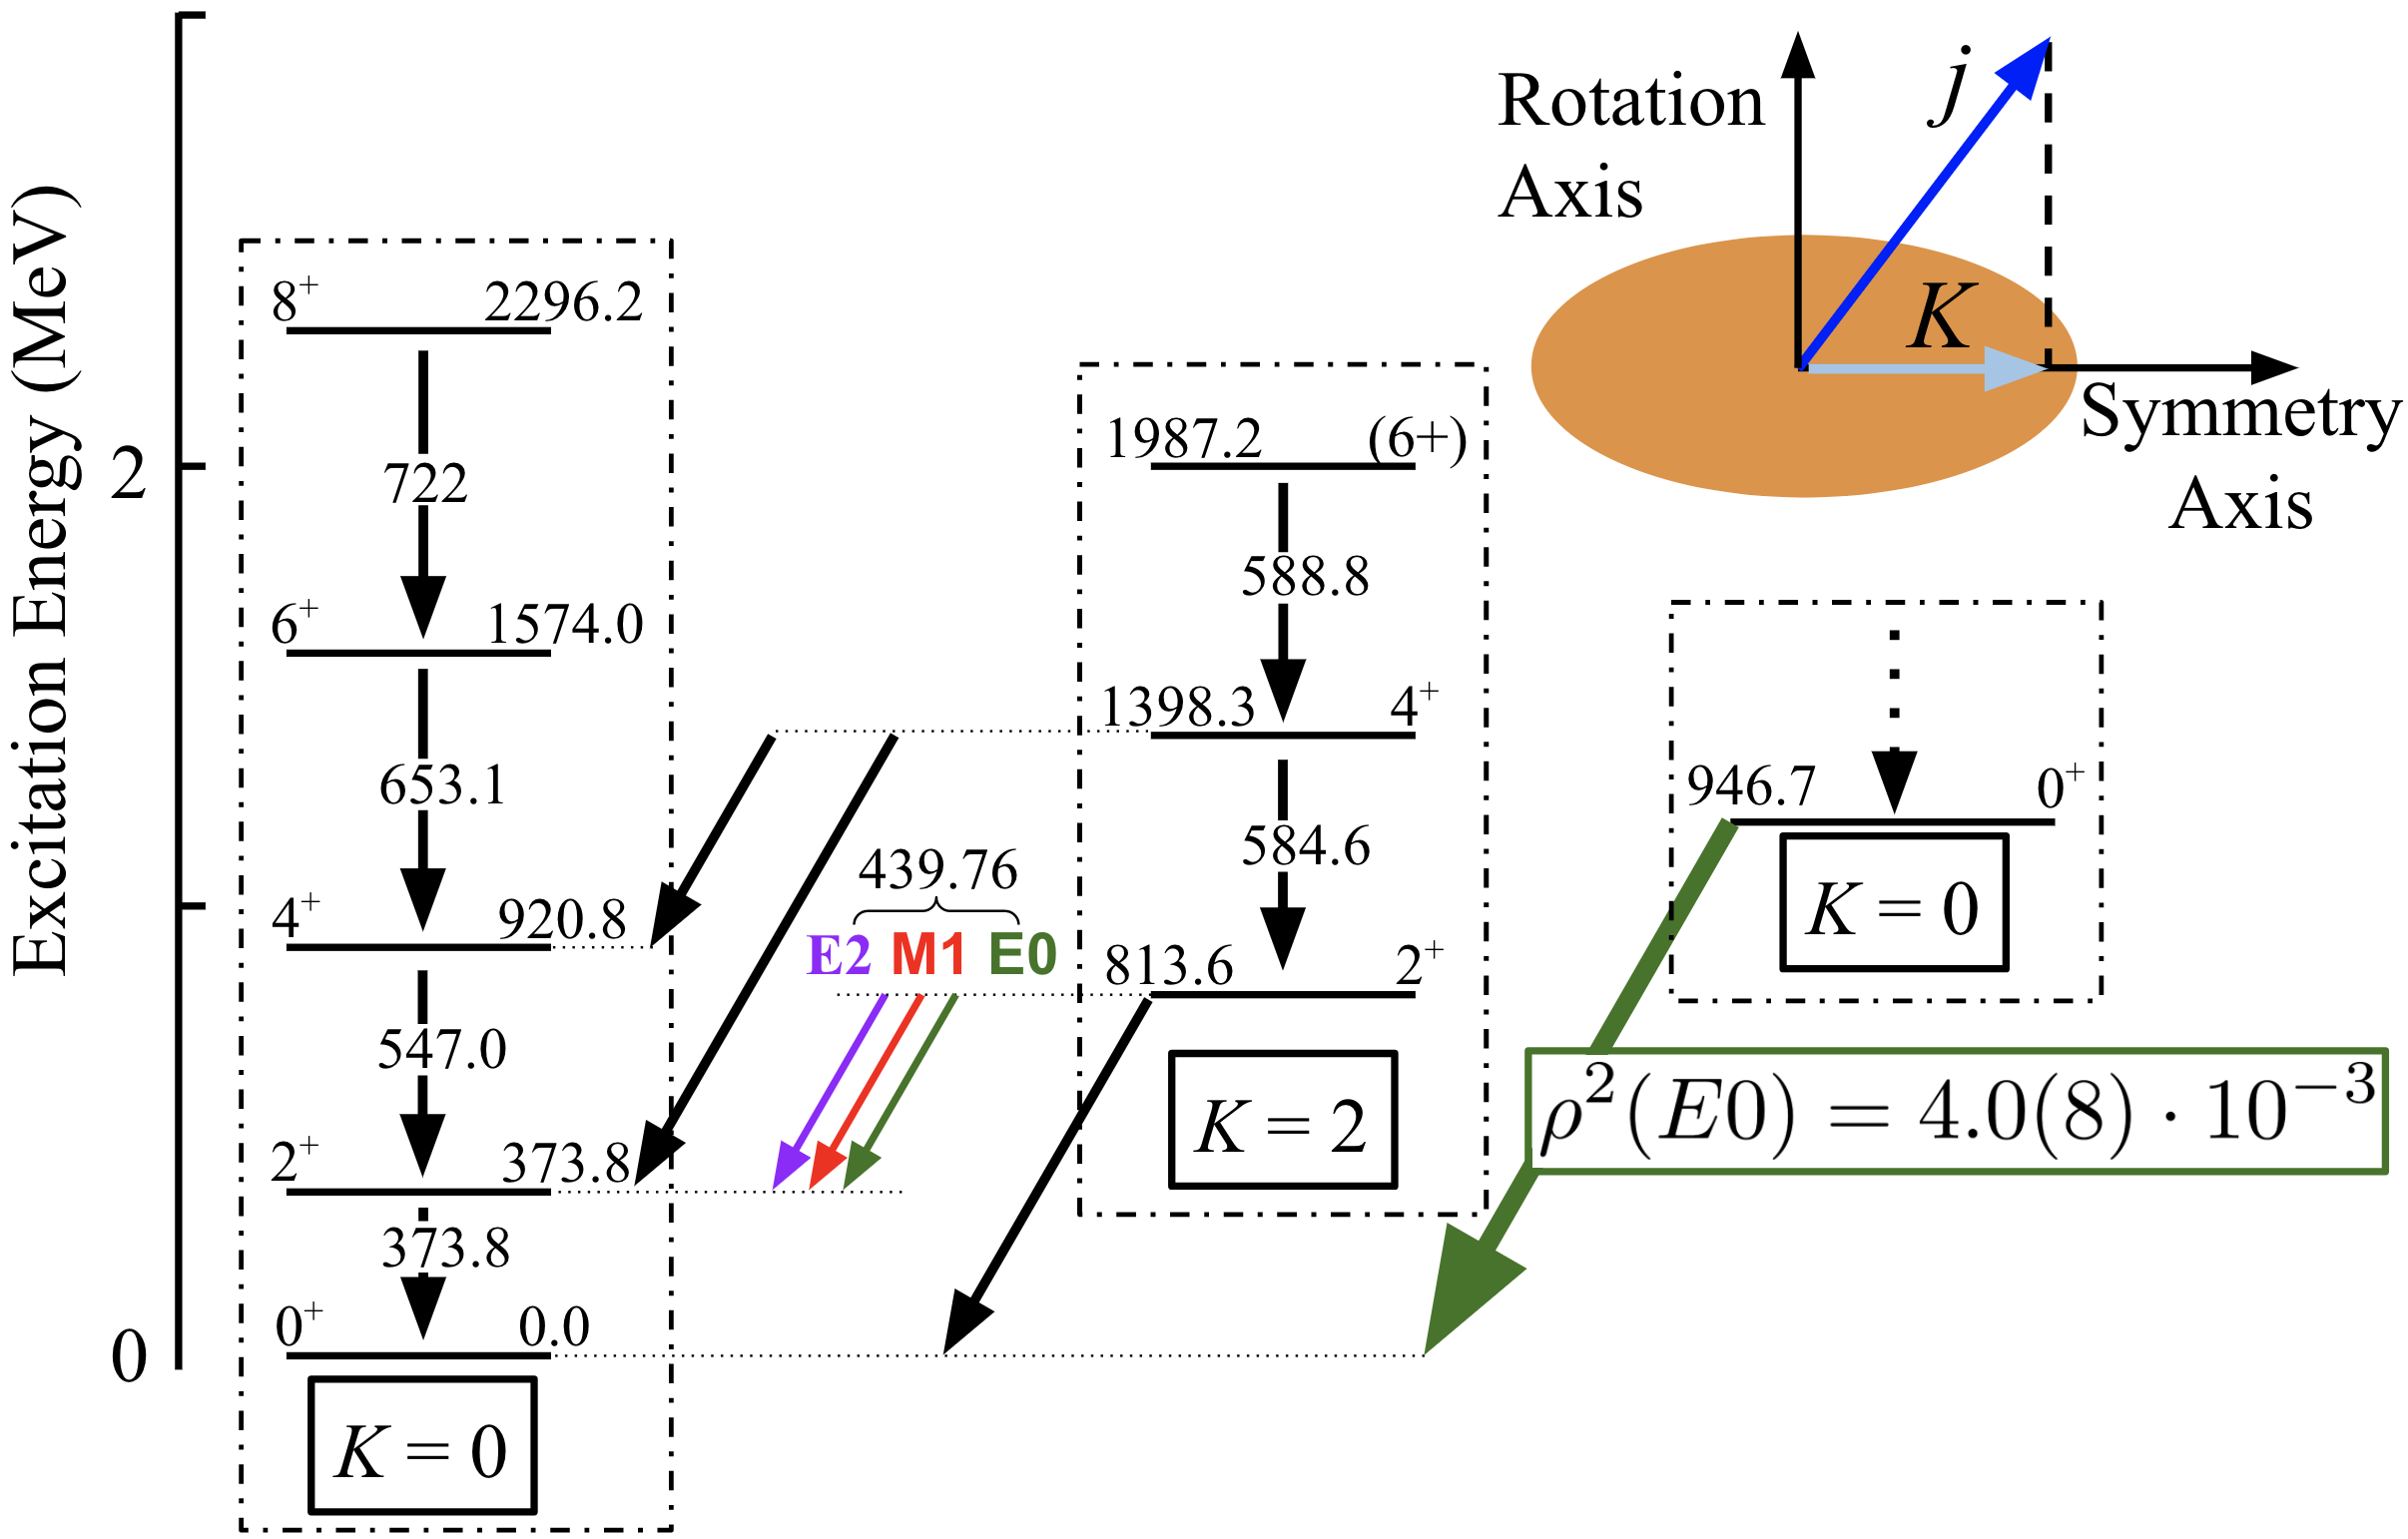
\includegraphics[width=\textwidth, keepaspectratio]{LevelsWithK.png}
\end{figure}
\end{frame}

%%%%%%%%%%%%%%%%%%%%%%%%%

%%%%%%%%%%%%%%%%%%%%%%%%%

\begin{frame}{Methods}
\framesubtitle{Internal Conversion Decay}
The electron carries away energy equal to the transition energy less the binding energy of the particular atomic orbital. i.e.
\begin{gather*}
T_e = T_\gamma - B_e
\label{iceEnergy}
\end{gather*}
Total decay probability as a sum of individual decay modes:
\begin{gather*}
\lambda_t = \lambda_\gamma + \lambda_e + ...
\end{gather*}
This can be rearranged as
\begin{gather*}
\lambda_t = \lambda_\gamma(1+\alpha_e + ...)
\end{gather*}
with
\begin{gather*}
 \alpha_e=\frac{\lambda_e}{\lambda_\gamma}
\end{gather*}
\end{frame}

%%%%%%%%%%%%%%%%%%%%%%%%%

%%%%%%%%%%%%%%%%%%%%%%%%%

\begin{frame}{Methods}
\framesubtitle{Measuring $\rho^2(E0)$}
\begin{figure}[!hht]
  \centering
  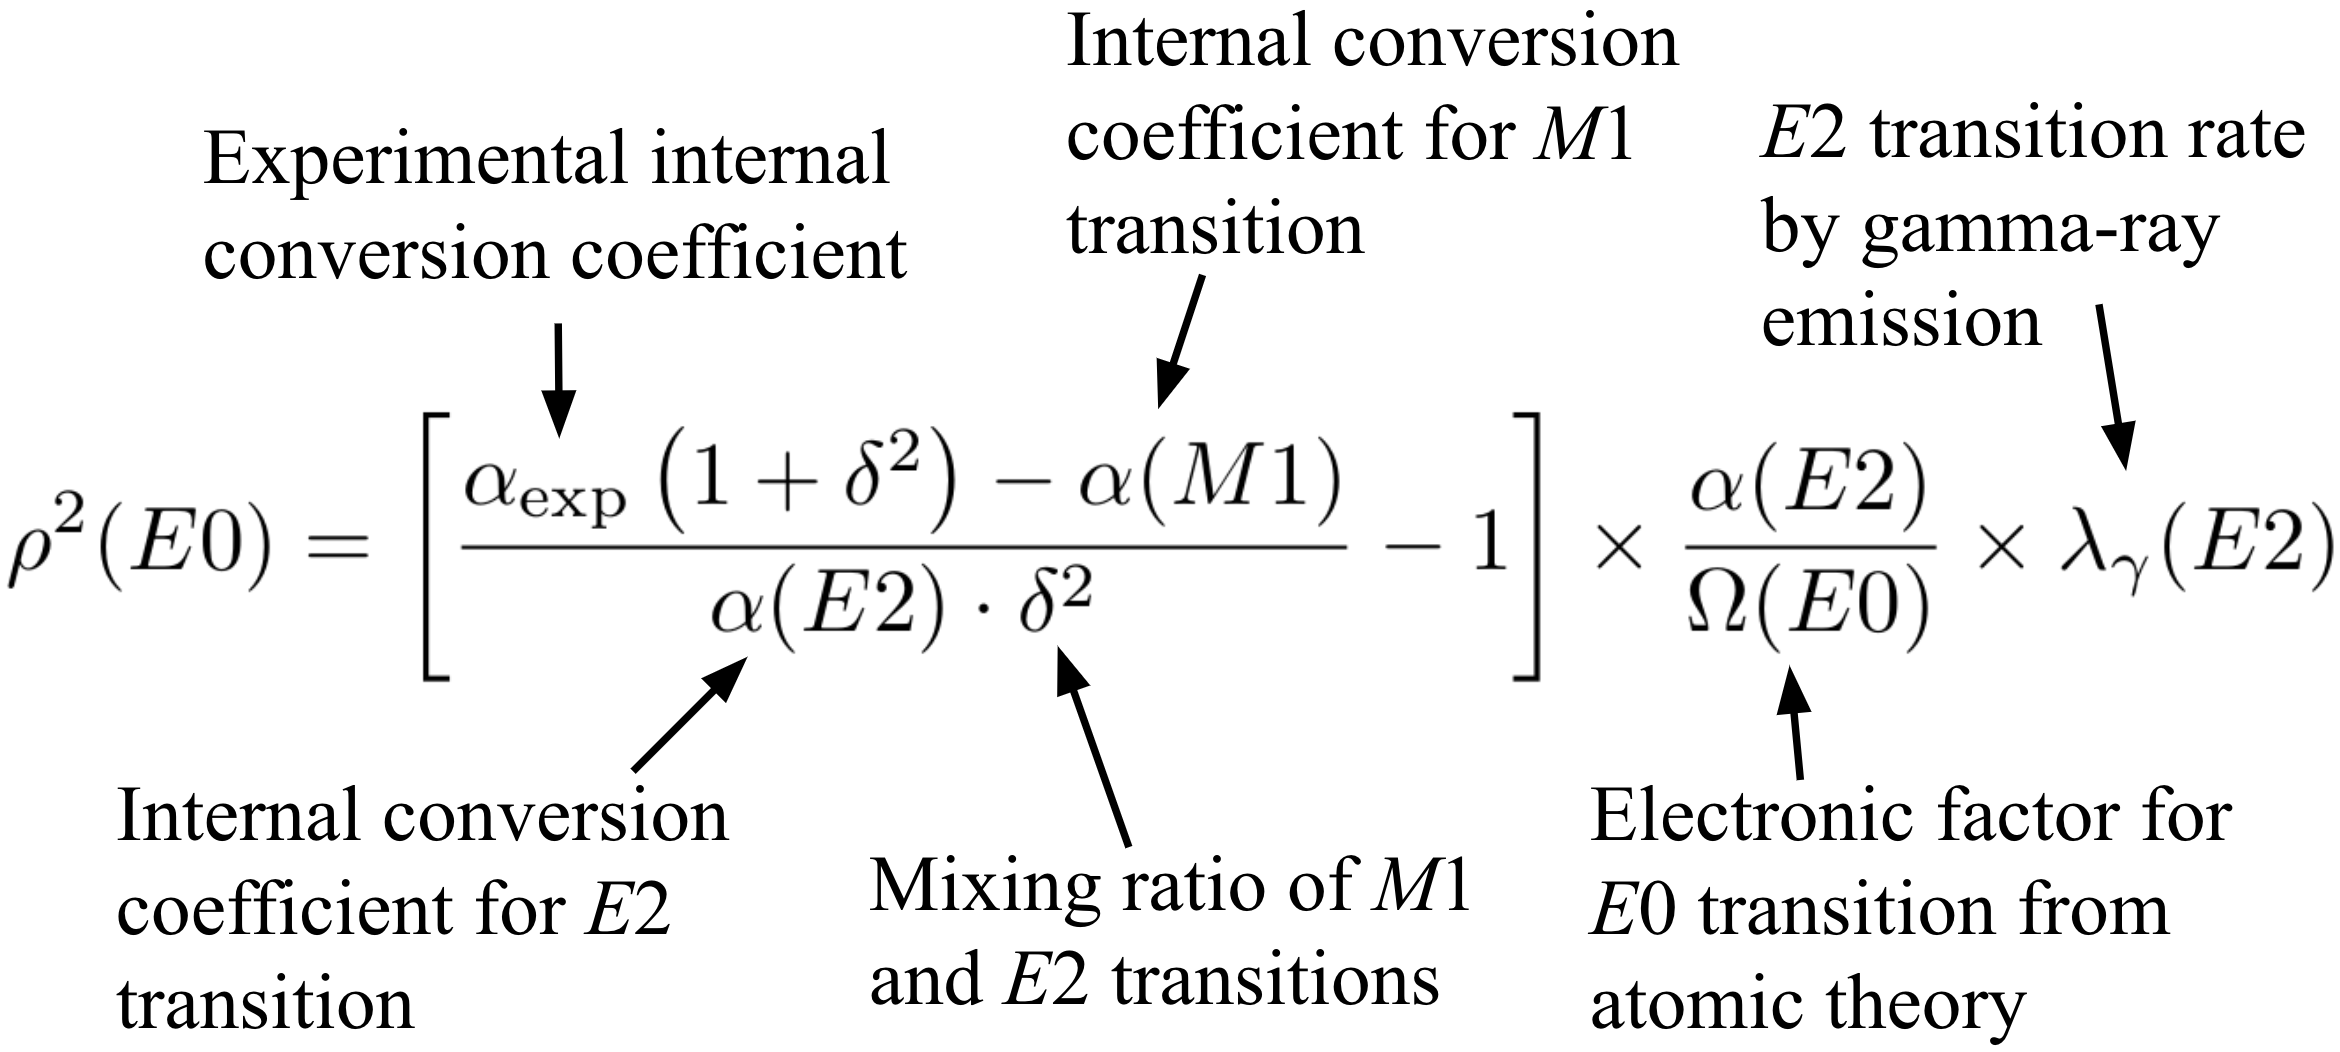
\includegraphics[width=\textwidth, keepaspectratio]{E0strengthDisambig.png}
\end{figure}
\end{frame}

%%%%%%%%%%%%%%%%%%%%%%%%%

%%%%%%%%%%%%%%%%%%%%%%%%%

\begin{frame}{Methods}
\framesubtitle{$\gamma$-ray Gating}
\begin{figure}[!hht]
  \centering
  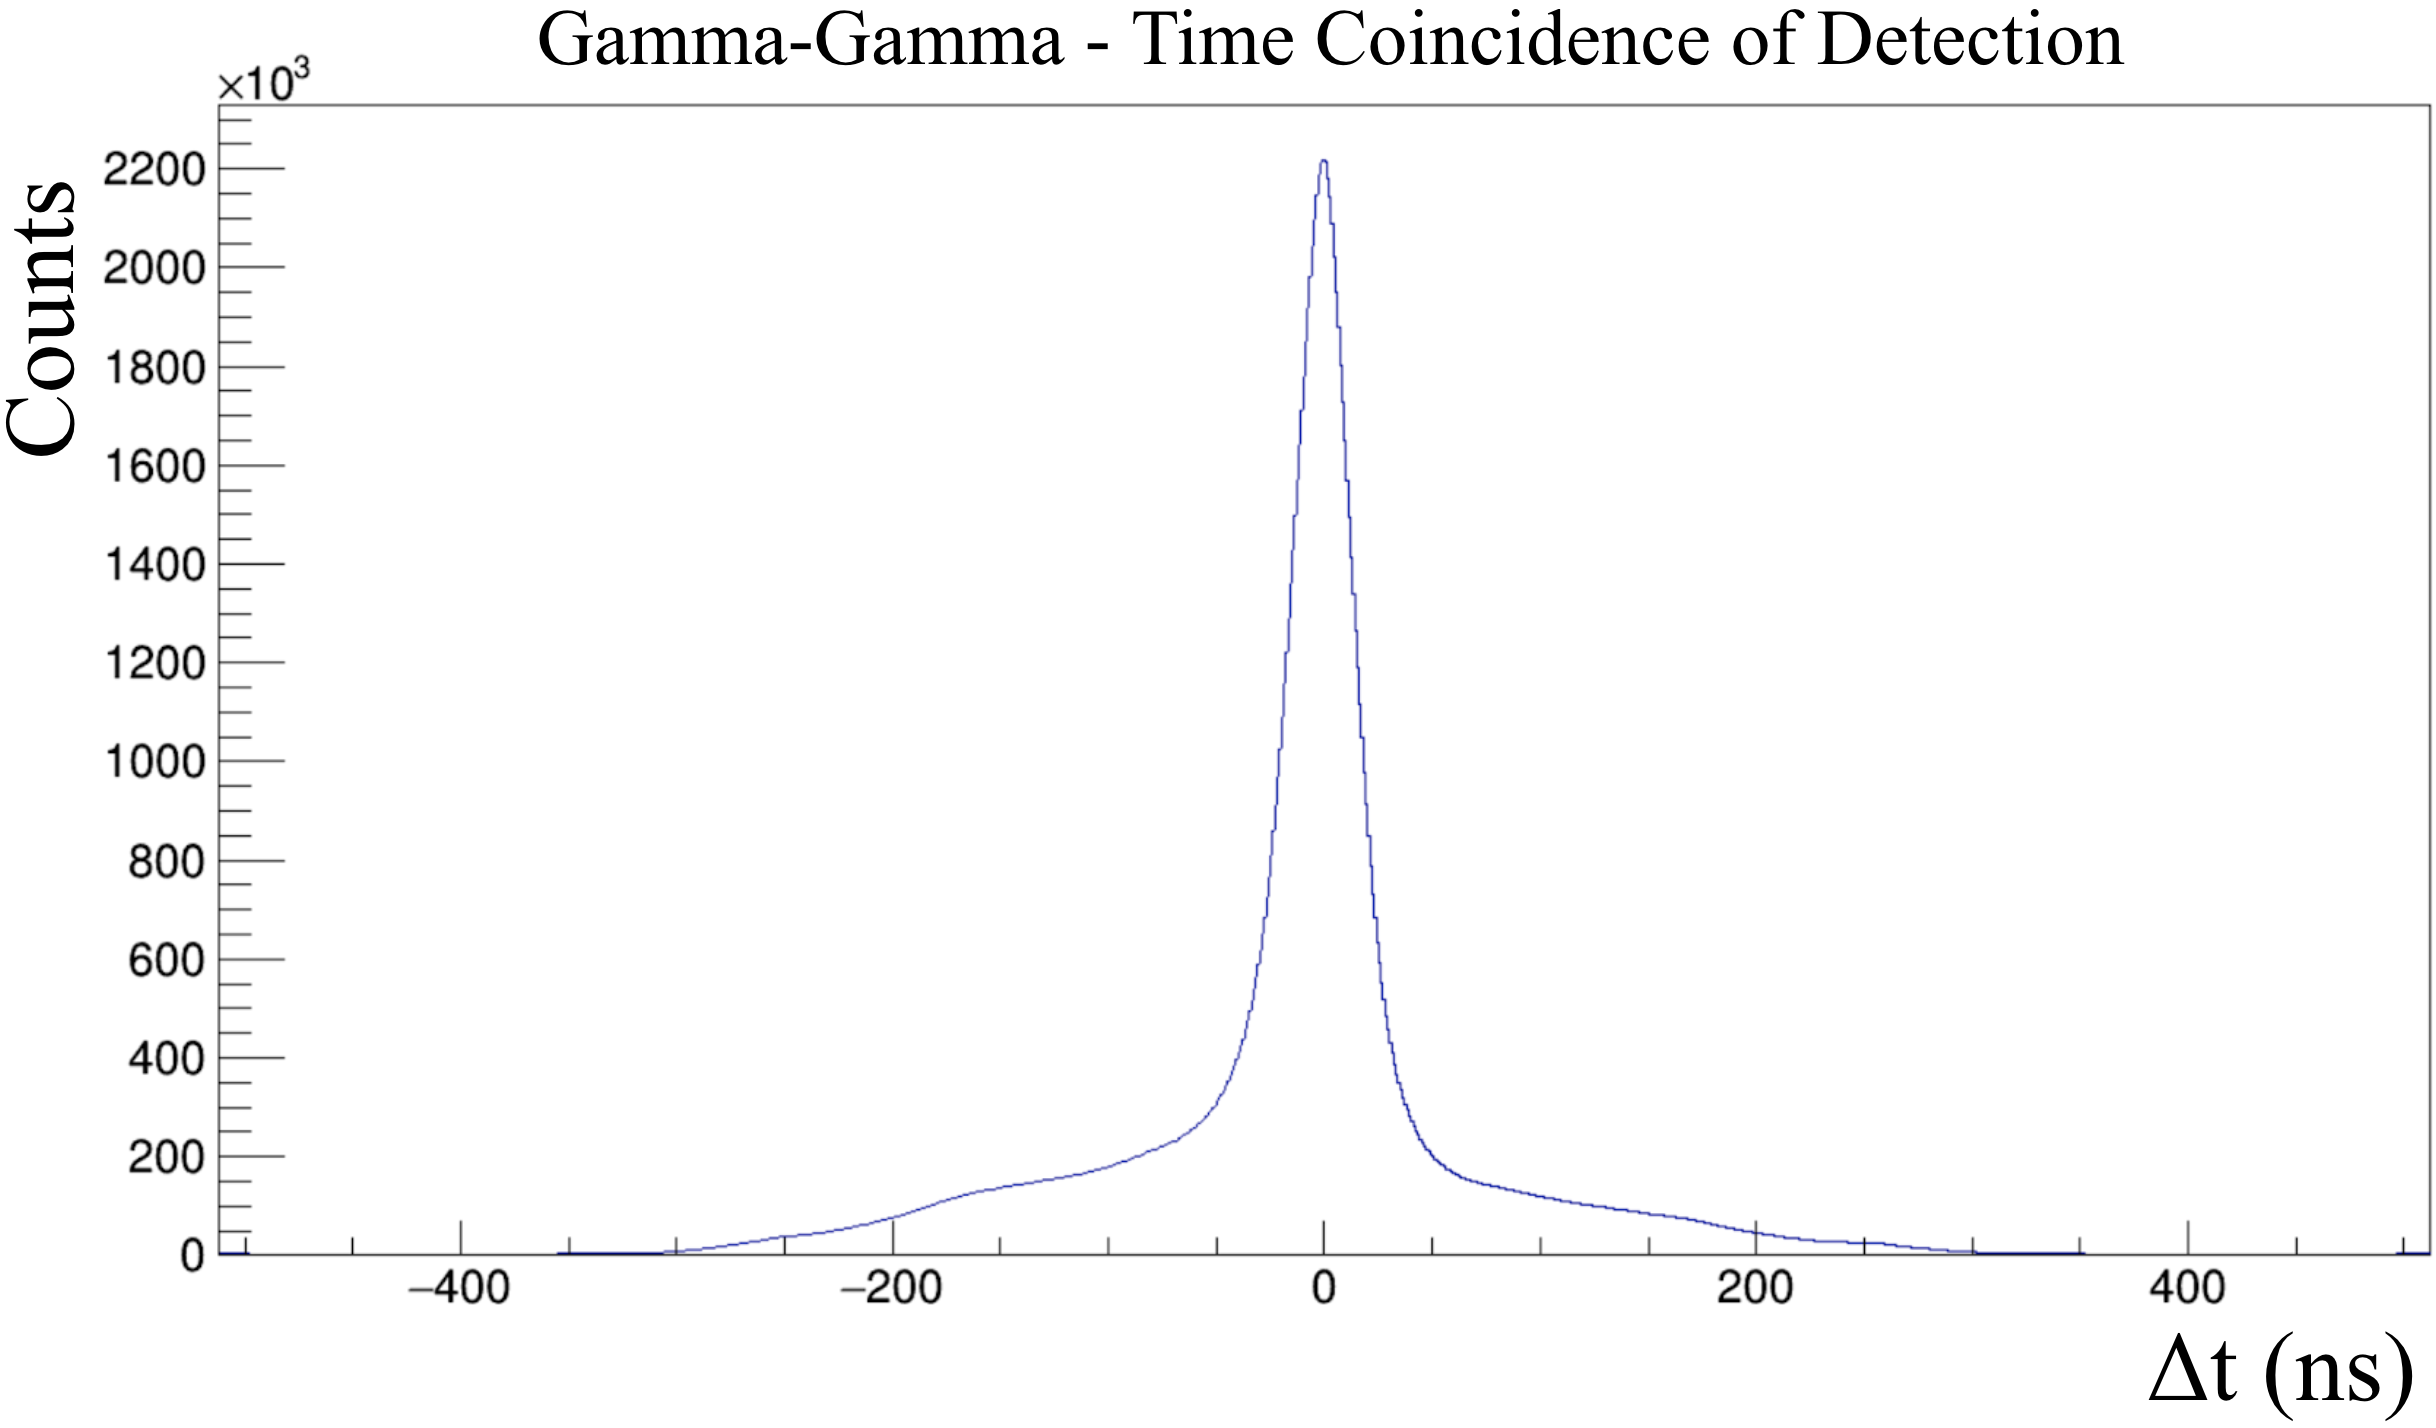
\includegraphics[width=0.9\textwidth, keepaspectratio]{GG_Gate1.png}
  \caption{Example of gamma-gamma time coincidence plot from detection by TIGRESS.}
  \label{yyHist}
\end{figure}
\end{frame}

%%%%%%%%%%%%%%%%%%%%%%%%%

%%%%%%%%%%%%%%%%%%%%%%%%%

\begin{frame}{Methods}
\framesubtitle{$\gamma$-ray Gating}
\begin{figure}[!hht]
  \centering
  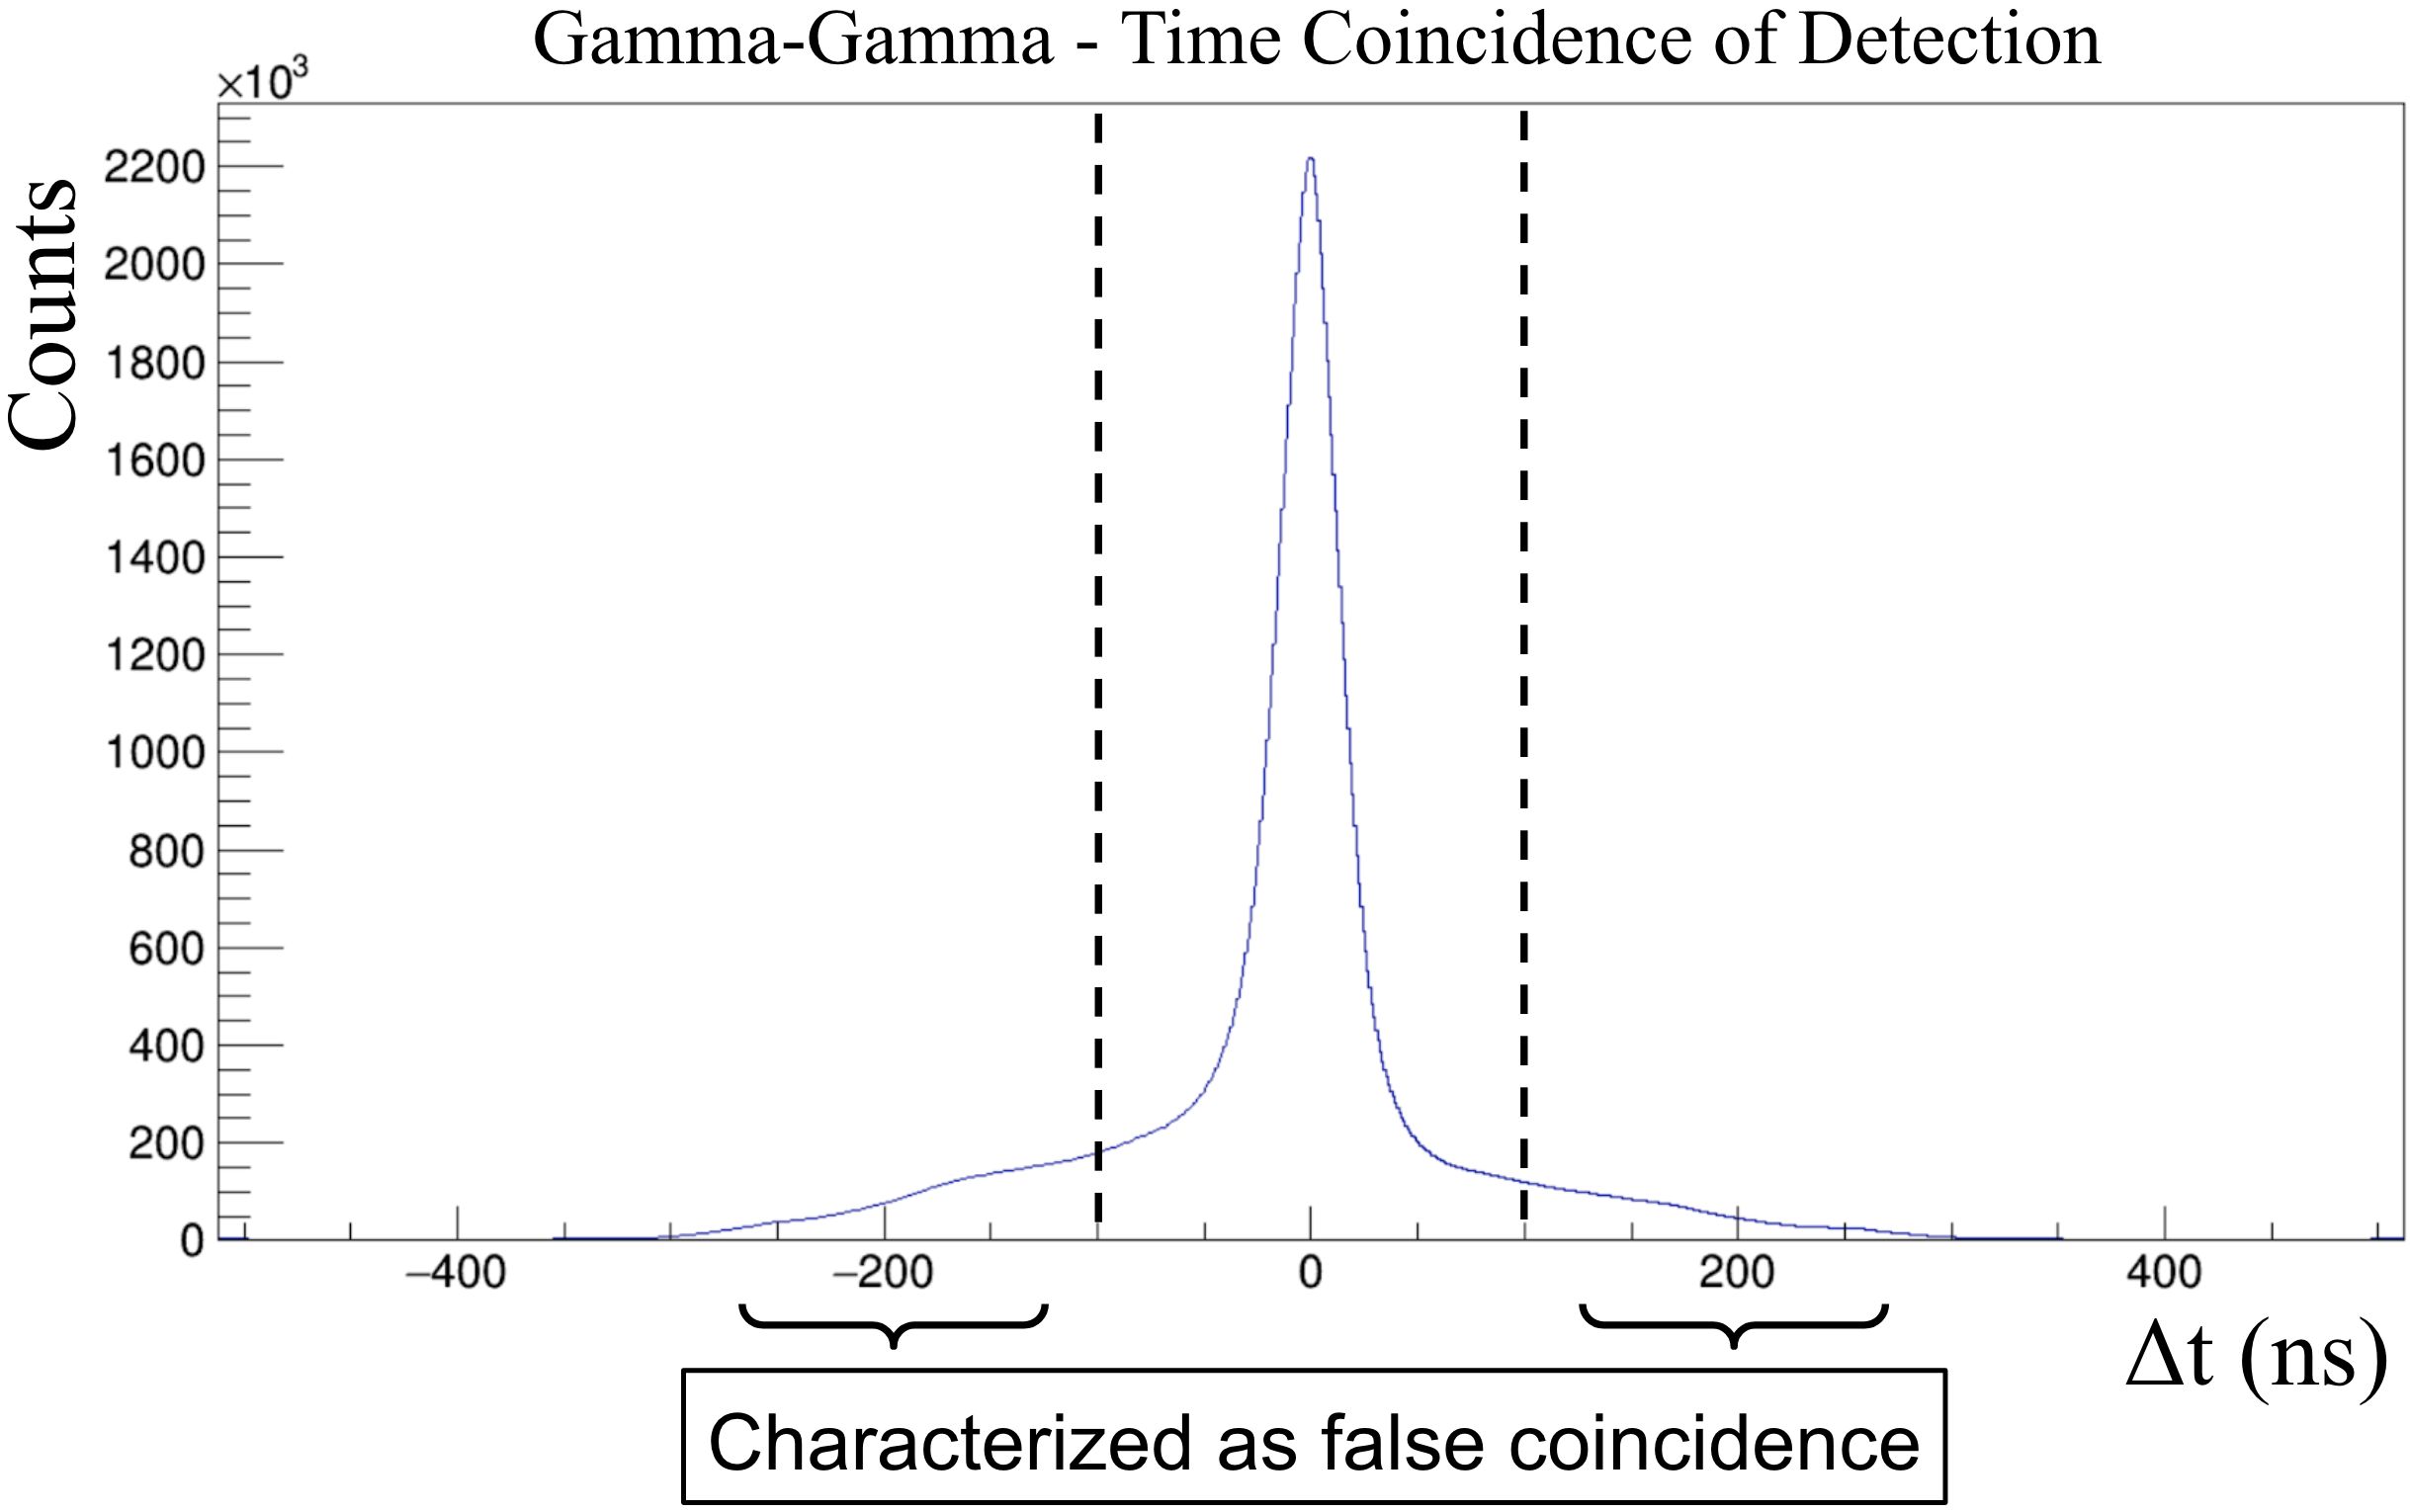
\includegraphics[width=0.9\textwidth, keepaspectratio]{GG_Gate2.png}
  \caption{Applying a narrow time 'gate' that restricts the definition of 'coincidence' for gamma ray detection.}
  \label{yyHist}
\end{figure}
\end{frame}

%%%%%%%%%%%%%%%%%%%%%%%%%

%%%%%%%%%%%%%%%%%%%%%%%%%

\begin{frame}{Methods}
\framesubtitle{$\gamma$-ray Gating}
\begin{figure}[!hht]
  \centering
  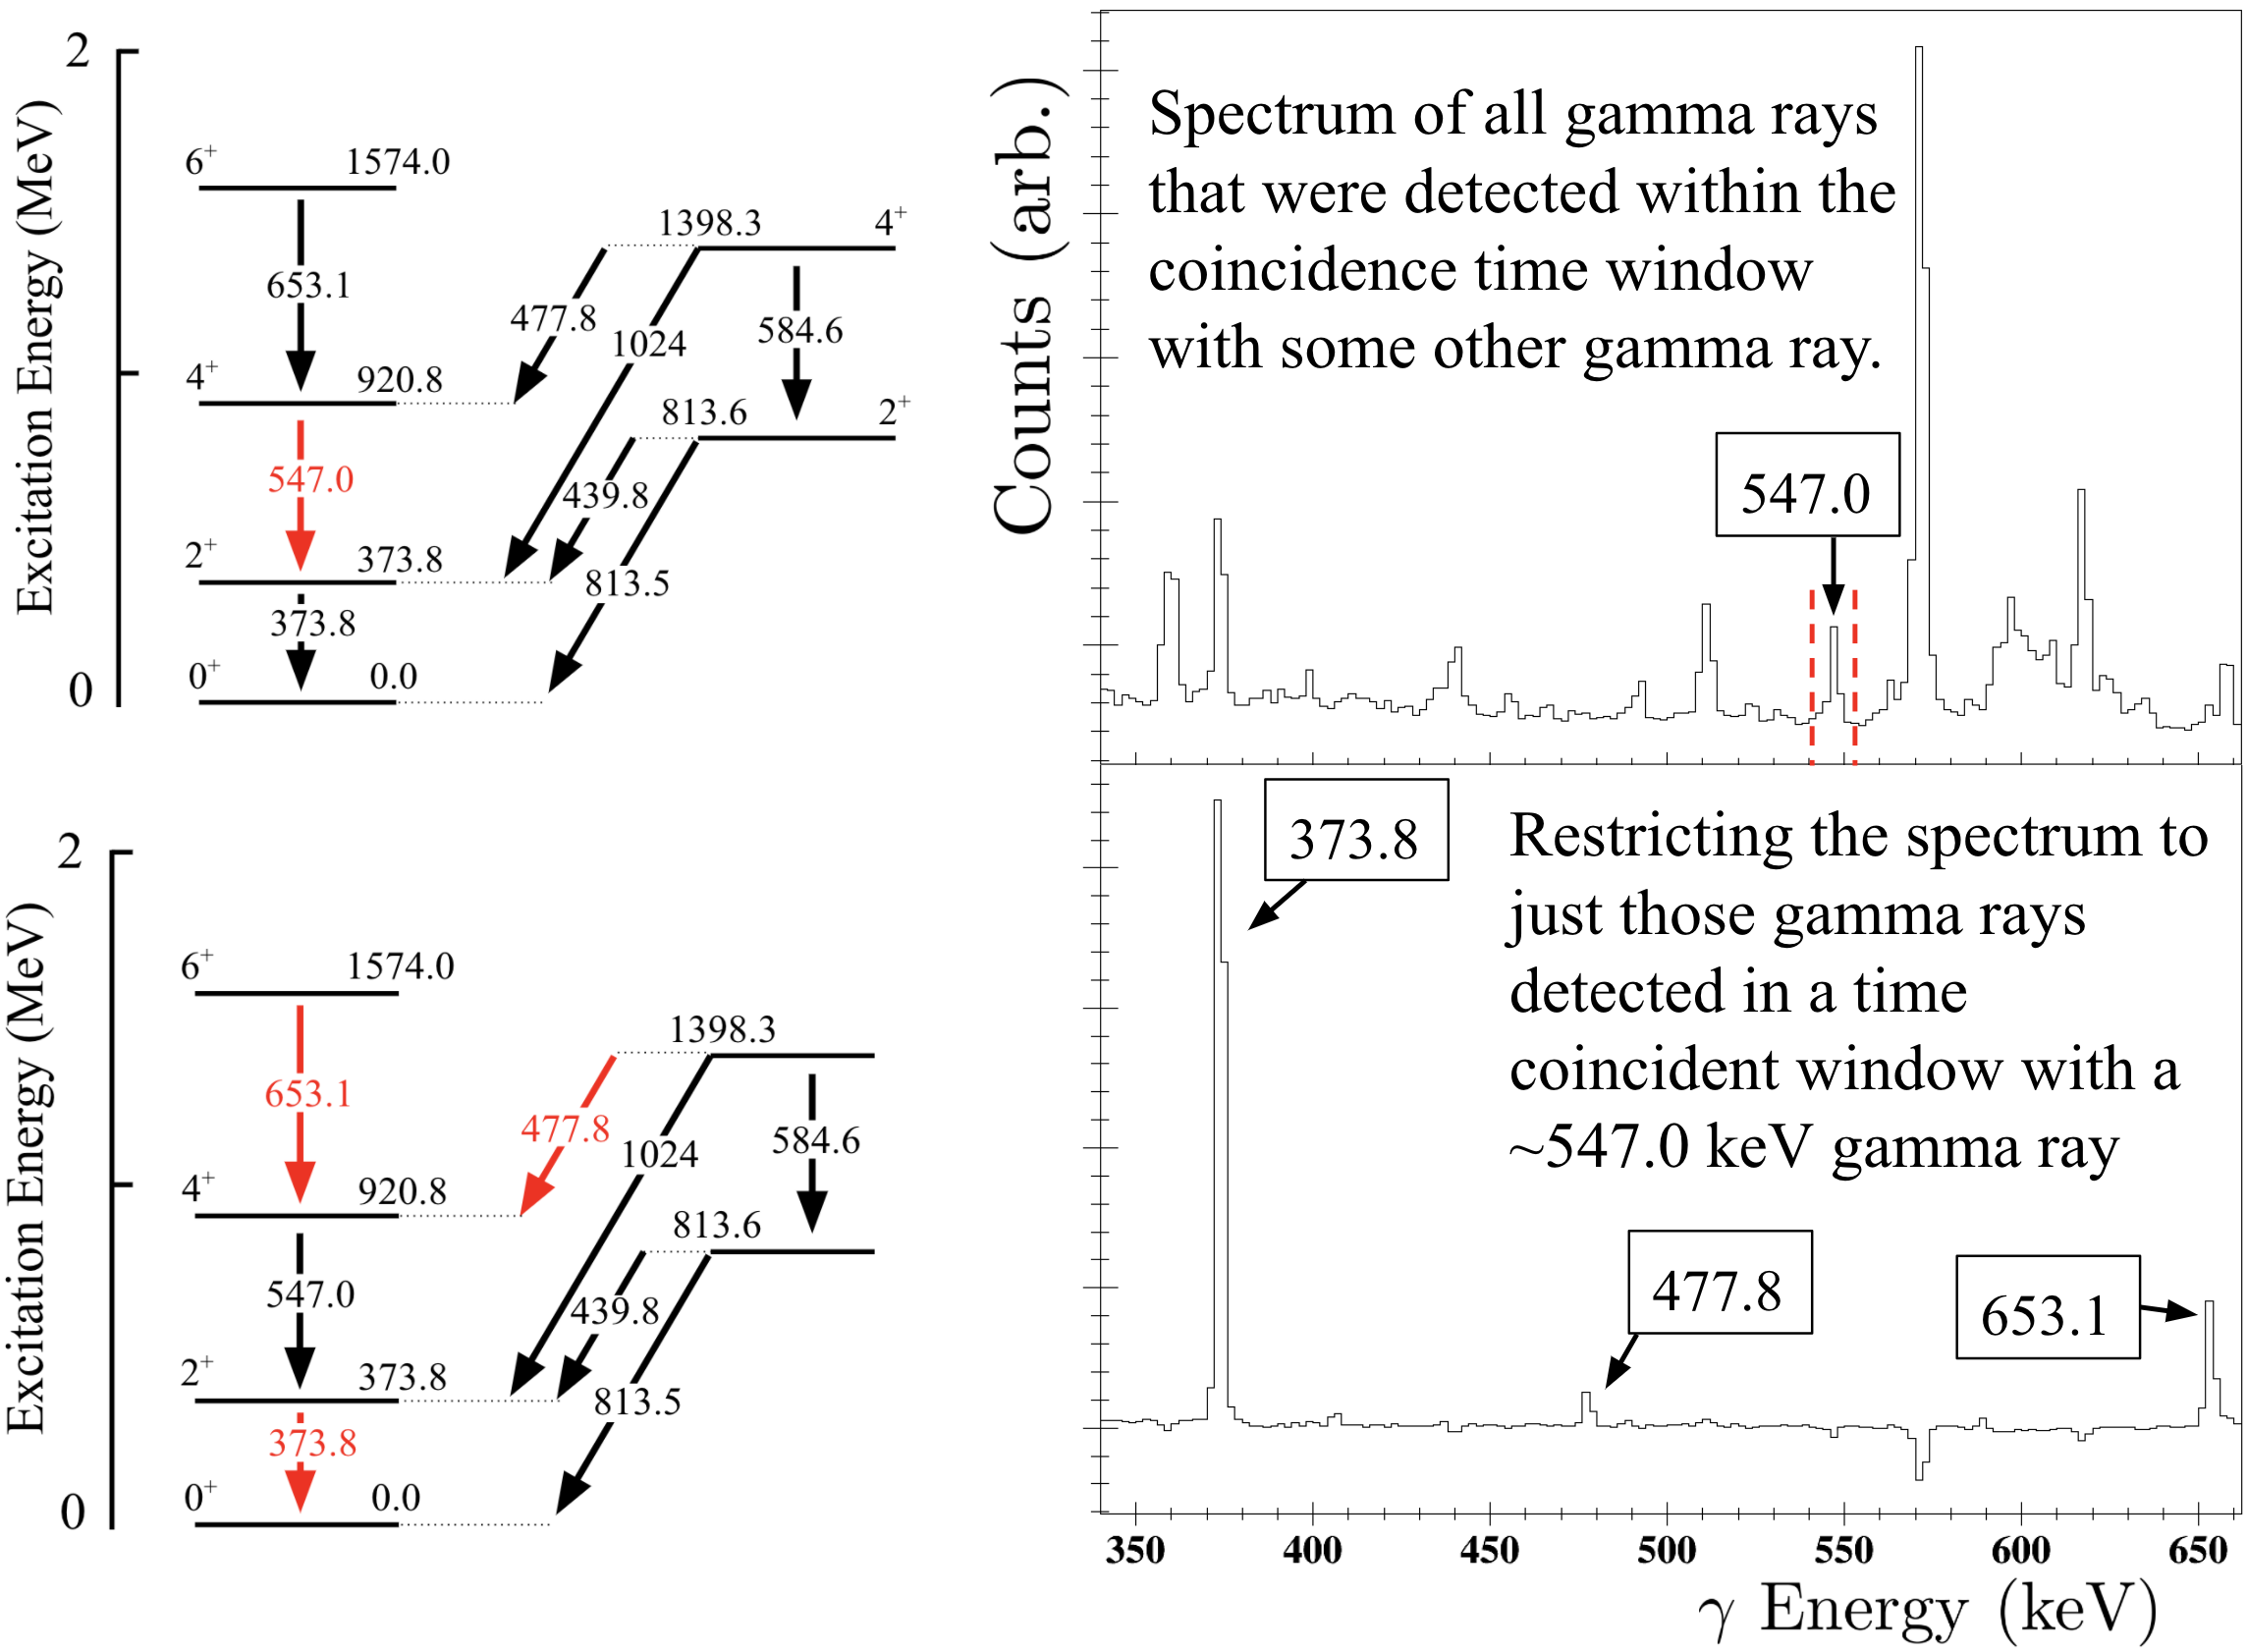
\includegraphics[width=0.93\textwidth, keepaspectratio]{CombinedGating.png}
  \label{GatedSpectra}
\end{figure}
\end{frame}


%%%%%%%%%%%%%%%%%%%%%%%%%

%%%%%%%%%%%%%%%%%%%%%%%%%

\begin{frame}{Methods}
\framesubtitle{Calculating the Internal Conversion Coefficient}
\begin{figure}[!hht]
  \centering
  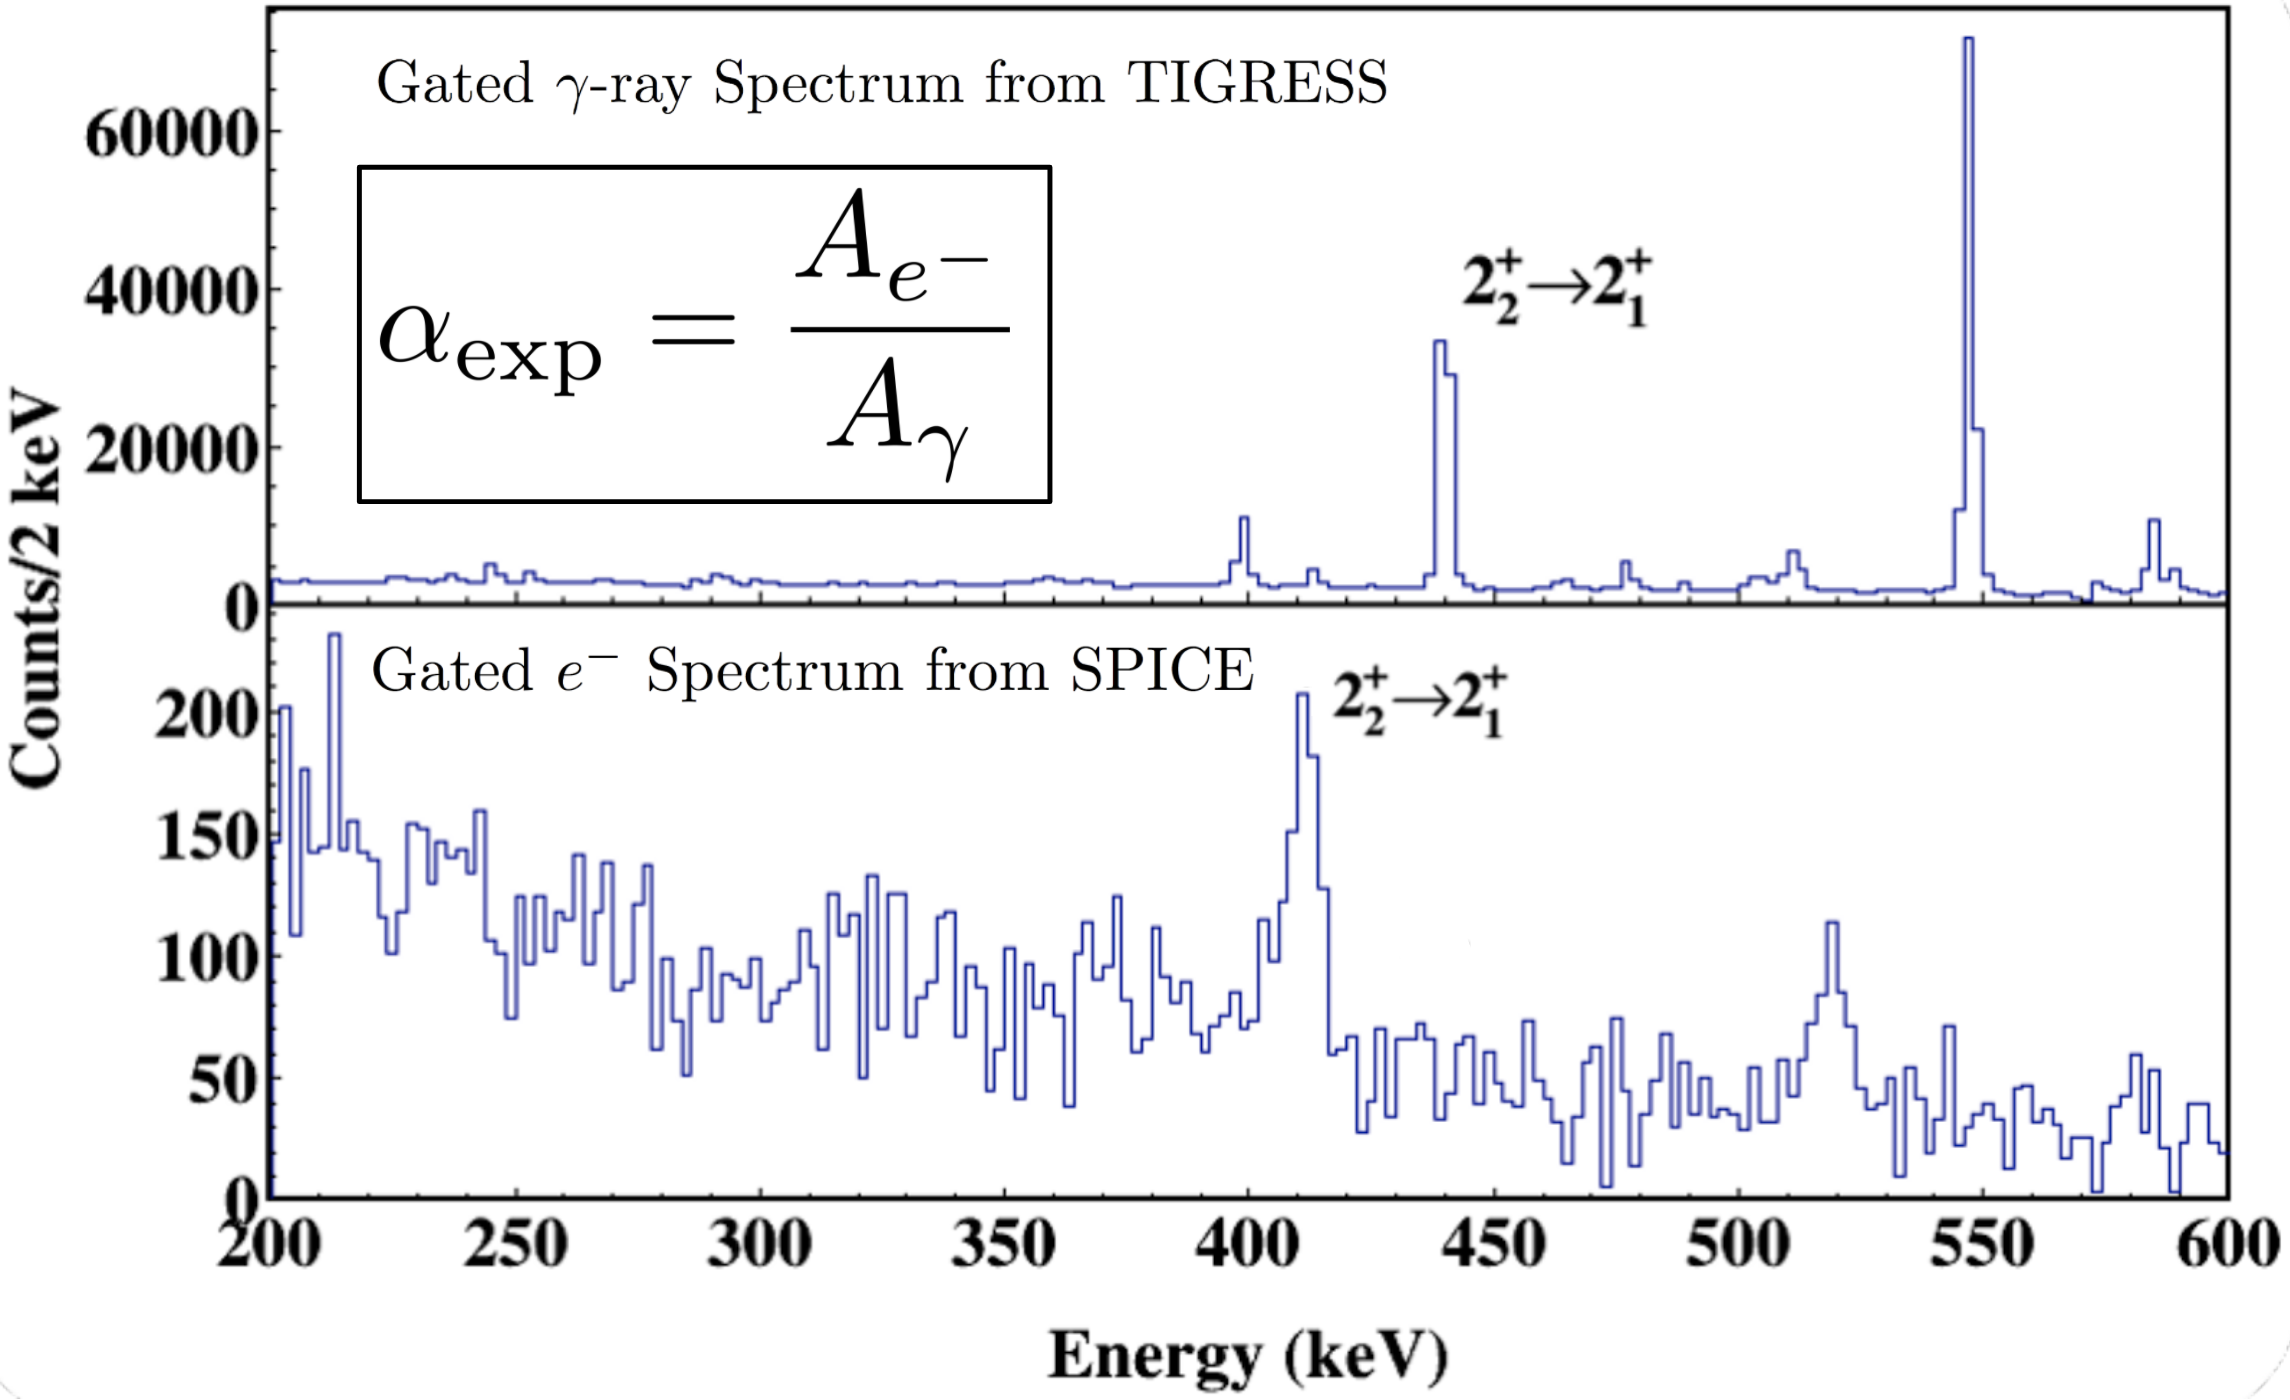
\includegraphics[width=\textwidth, keepaspectratio]{JTSStack.png}
  \caption{Example of $\gamma$ ray and electron spectra from the $^{110}\mathrm{Pd}$ data set.}
  \label{comparison}
\end{figure}
\end{frame}


%%%%%%%%%%%%%%%%%%%%%%%%%

%%%%%%%%%%%%%%%%%%%%%%%%%

\begin{frame}{Methods}
\framesubtitle{Putting it all together: $\rho^2(E0)$}
\begin{figure}[!hht]
  \centering
  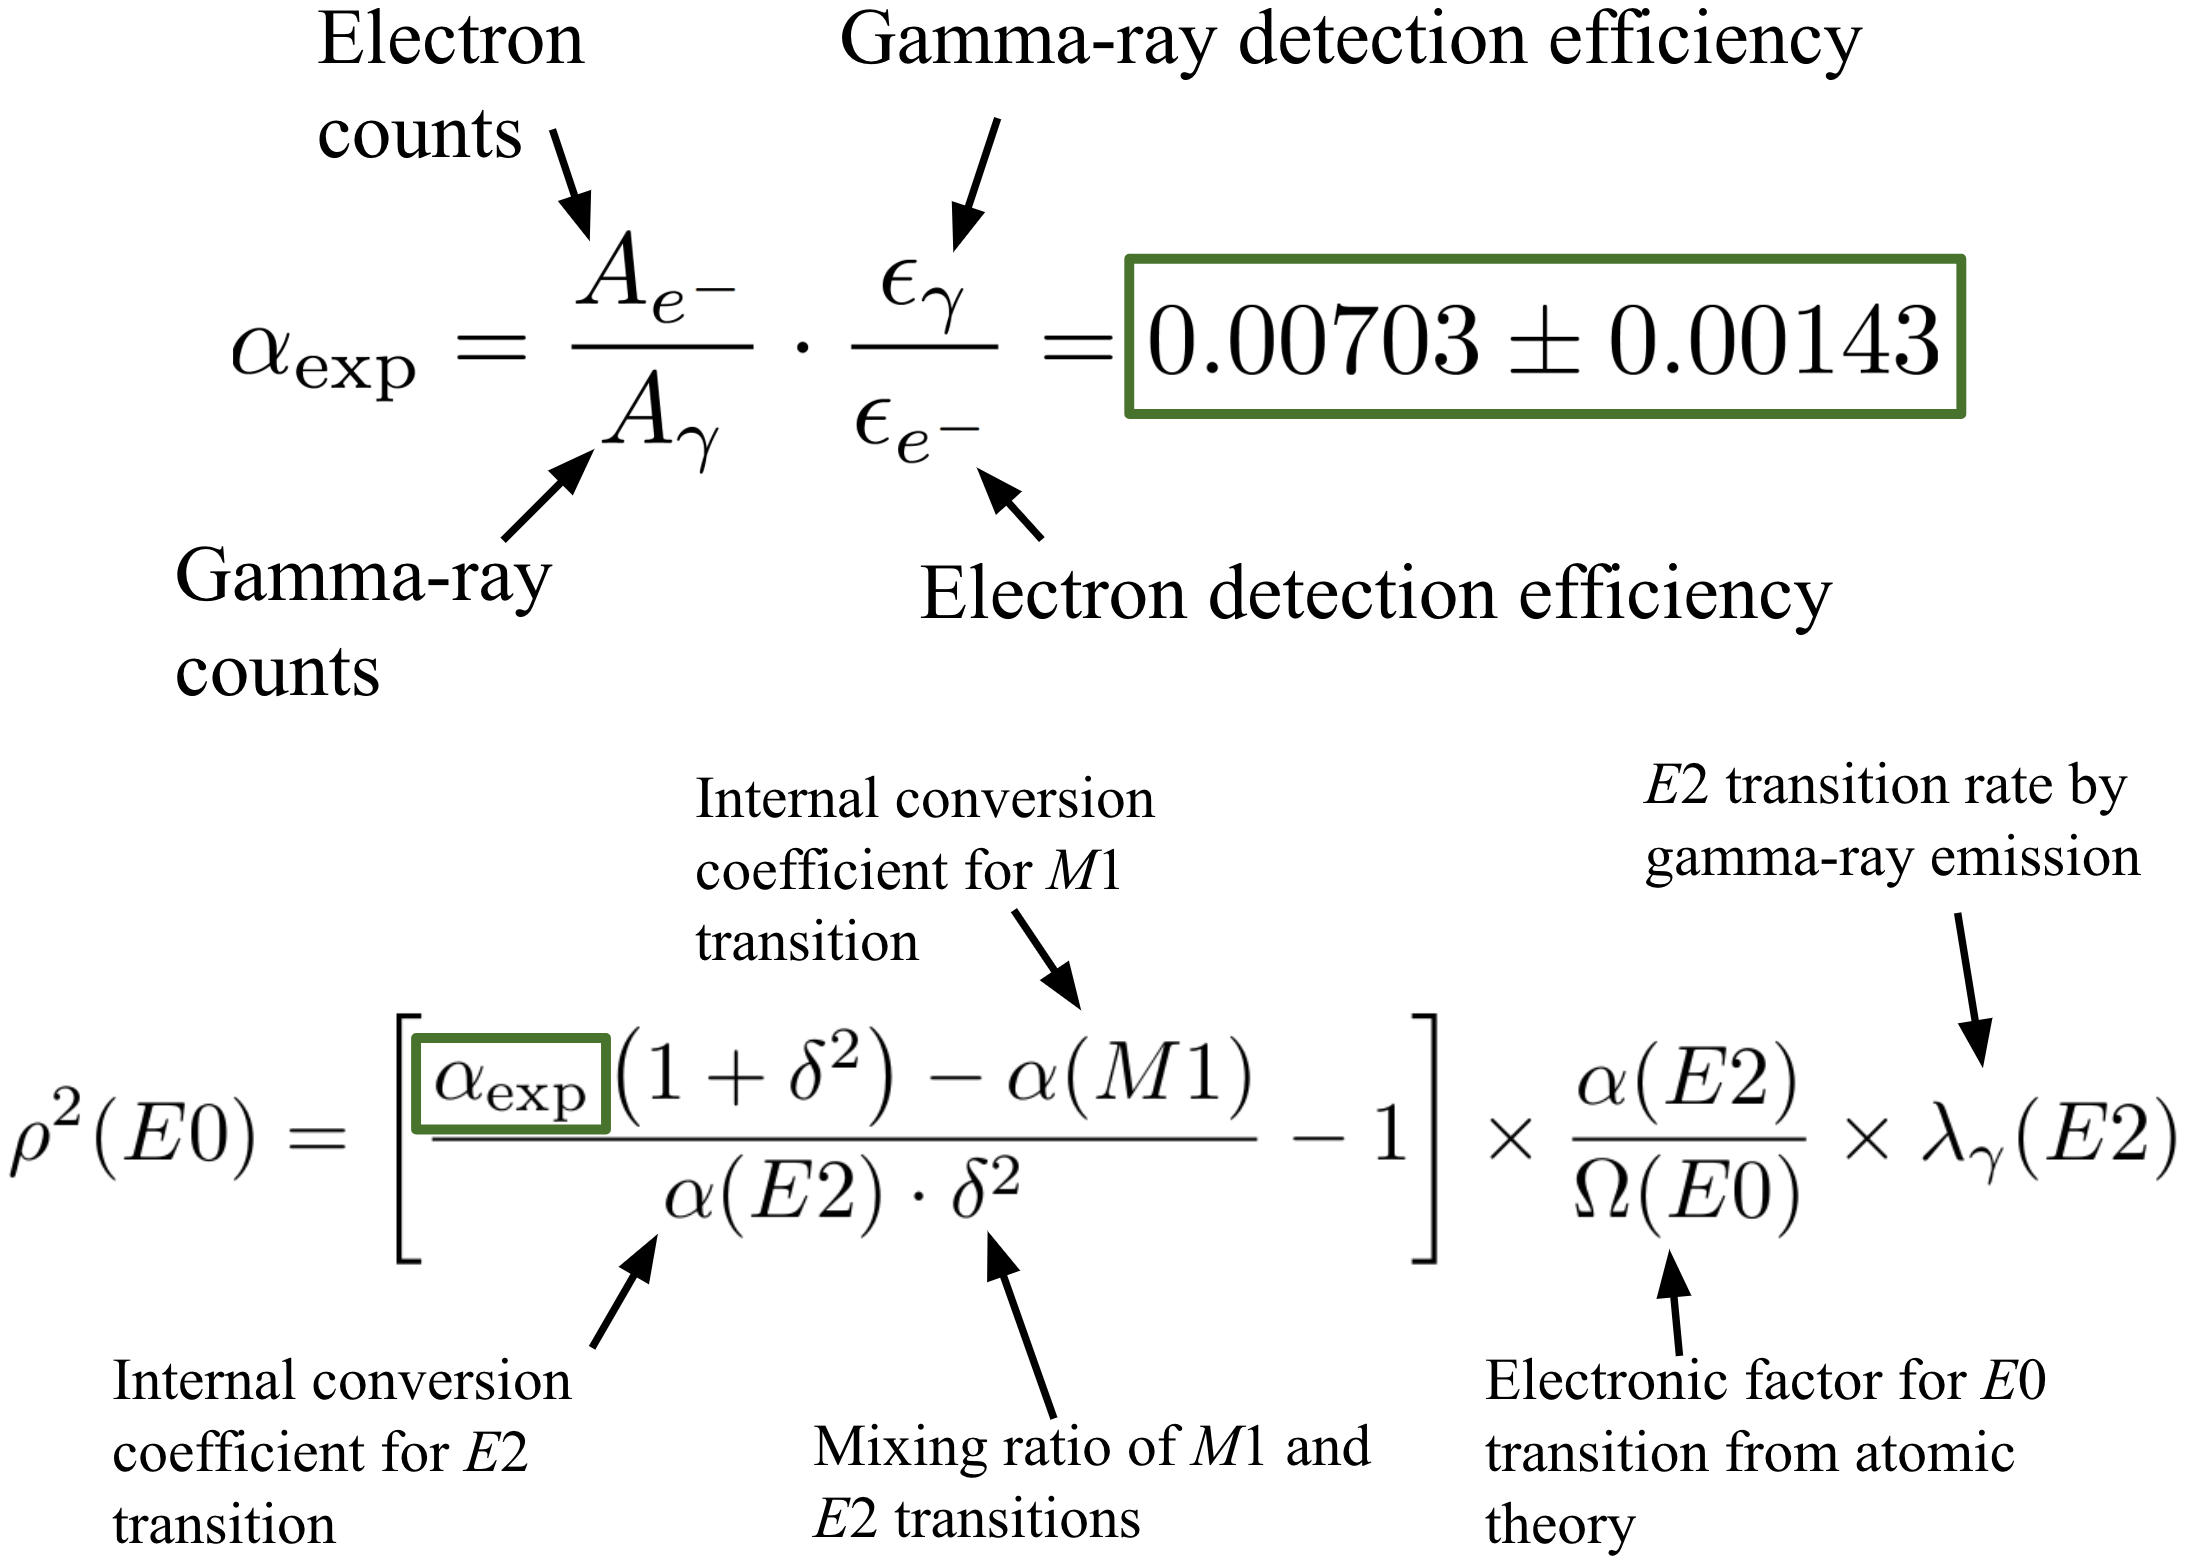
\includegraphics[width=\textwidth, keepaspectratio]{AllTogether.png}
\end{figure}
\end{frame}

\section{Results: $\rho^2(E0)$ Measurement Limit}

%%%%%%%%%%%%%%%%%%%%%%%%% 

%%%%%%%%%%%%%%%%%%%%%%%%%

\begin{frame}{Results}
\framesubtitle{Error Analysis}
Some input variables have large, asymmetric error bars, \newline
e.g. $\delta = -4.6^{+1.9}_{-1.2}$
\begin{figure}[!hht]
  \centering
  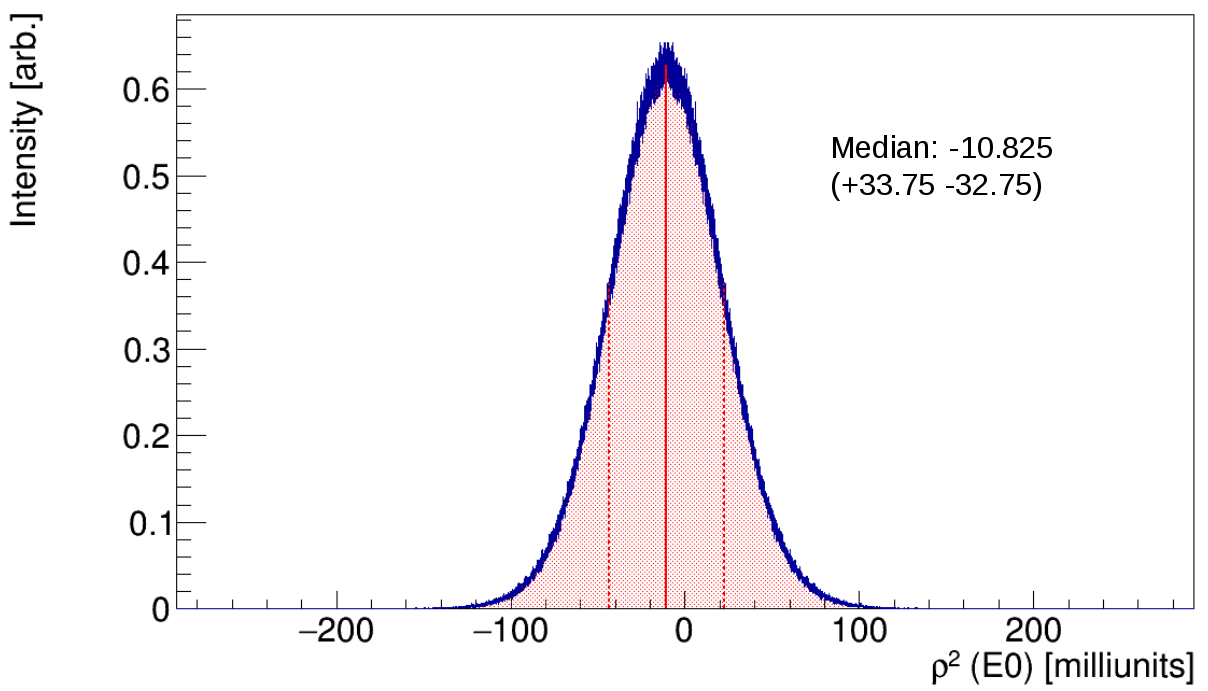
\includegraphics[width=0.8\textwidth, keepaspectratio]{MonteCarlo.png}
  \caption{An example distribution of $\rho^2(E0)$ for the $2^+_2 \rightarrow 2^+_1$ transition in $^{110}\mathrm{Pd}$, produced by the Monte Carlo method.}  \label{MonteCarloSim}
\end{figure}
\end{frame}

%%%%%%%%%%%%%%%%%%%%%%%%%

%%%%%%%%%%%%%%%%%%%%%%%%%

\begin{frame}{Results}
\framesubtitle{Neyman Construction}
\begin{figure}[!hht]
  \centering
  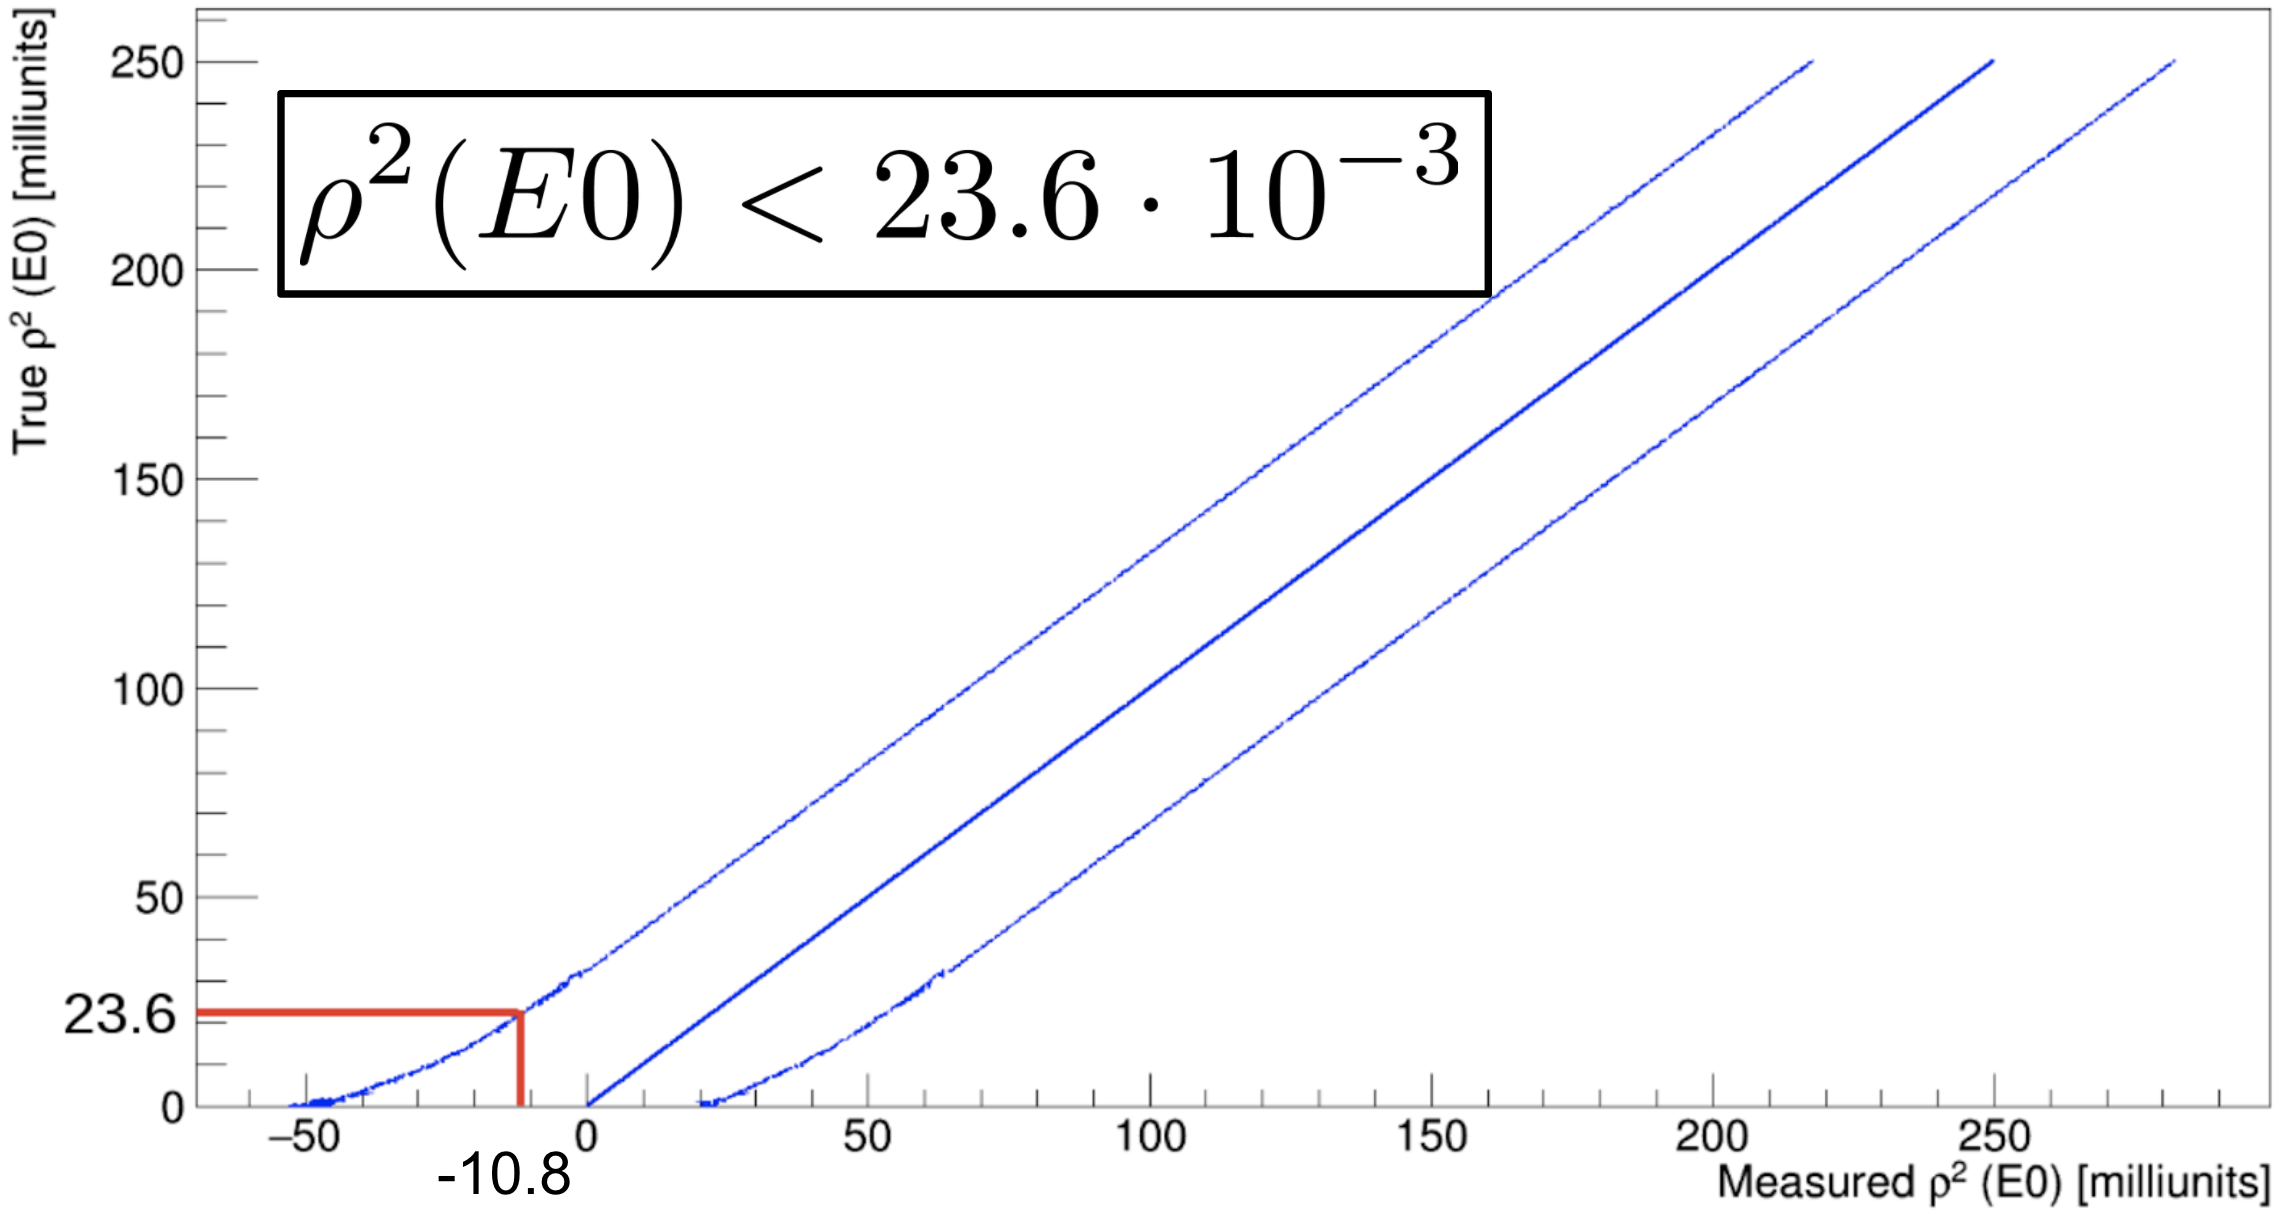
\includegraphics[width=\textwidth, keepaspectratio]{NeymanAndFinal.png}
  \caption{A Neyman construction using the distribution of Figure \ref{MonteCarloSim} from the previous slide.}
  \label{Neyman}
\end{figure}
\end{frame}

%%%%%%%%%%%%%%%%%%%%%%%%%


%%%%%%%%%%%%%%%%%%%%%%%%%

\begin{frame}{Results}
\framesubtitle{The Measurement in Context; Conclusion}

\begin{table}[h!]
\centering
 \begin{tabular}{||c c c c||} 
 \hline
 Nuclide & Level (keV) & $J_i^\pi \rightarrow J_f^\pi$ & $10^3 \times \rho^2(E0)$ \\ [0.5ex] 
 \hline\hline
  $^{104}\mathrm{Pd}$ & 1333.6 & $0^+_2 \rightarrow 0^+_1$ & $6(4)$  \footnotemark[1] \\
\hline
 $^{106}\mathrm{Pd}$ & 1133.9 & $0^+_2 \rightarrow 0^+_1$ & $14(4)$  \footnotemark[2] \\ 
\hline
 $^{106}\mathrm{Pd}$ & 1562.2 & $2^+_3 \rightarrow 2^+_1$ & $34(22)$  \footnotemark[2] \\
\hline
 $^{106}\mathrm{Pd}$ & 1706.4 & $0^+_3 \rightarrow 0^+_1$ & $< 3$  \footnotemark[2] \\
\hline
 $^{106}\mathrm{Pd}$ & 1909.5 & $2^+_4 \rightarrow 2^+_1$ & $21^{+10}_{-21}$  \footnotemark[2] \\
\hline
  $^{106}\mathrm{Pd}$ & 2242.5 & $2^+_5 \rightarrow 2^+_2$ & $96^{+43}_{-61}$  \footnotemark[2] \\ 
\hline
  $^{108}\mathrm{Pd}$ & 1052.8 & $0^+_2 \rightarrow 0^+_1$ & $< 3$  \footnotemark[1] \\
\hline
  $^{110}\mathrm{Pd}$ & 946.7 & $0^+_2 \rightarrow 0^+_1$ & $4.0 (8)$  \footnotemark[1] \\
\hline
  $^{110}\mathrm{Pd}$ & 813.6 & $2^+_2 \rightarrow 2^+_1$ & $< 26.3$  \\ [1ex] 
 \hline
 \end{tabular}
\end{table}

\footnotetext[1]{T. Kib\'edi and R.H. Spear, \textit{Atomic Data and Nuclear Data Tables.} 89 (2005) 77-100.}
\footnotetext[2]{E.E. Peters et al. \textit{Eur. Phys. J. A.} (2016) 52: 96.}
\end{frame}

%%%%%%%%%%%%%%%%%%%%%%%%%

%%%%%%%%%%%%%%%%%%%%%%%%%

\begin{frame}{Acknowledgements}
  \begin{block}{List of Collaborators}
  	Reiner Kruecken\footnotemark[1], James Smallcombe\footnotemark[1], 	Adam Garnsworthy\footnotemark[1], C.~Andreoiu\footnotemark[2], R.~Caballero-Folch\footnotemark[1], T.E.~Drake\footnotemark[3], L.J.~Evitts\footnotemark[1], G.~Hackman\footnotemark[1], J.~Henderson\footnotemark[1], A.~Kurkjian\footnotemark[1], M.~Moukaddam\footnotemark[1], B.~Olaizola\footnotemark[1], E.E.~Peters\footnotemark[4], D.~Southall\footnotemark[1], P.~Ruotsalainen\footnotemark[1], C.E.~Svensson\footnotemark[5], M.~Wiens\footnotemark[1], S.W.~Yates\footnotemark[4], T.~Zidar\footnotemark[5].
  \end{block}
\footnotetext[1]{TRIUMF}
\footnotetext[2]{Department of Chemistry, Simon Fraser University}
\footnotetext[3]{Department of Physics, University of Toronto}
\footnotetext[4]{Department of Chemistry and Physics \& Astronomy, University of Kentucky}
\footnotetext[5]{Department of Physics, University of Guelph}
\end{frame}

\end{document}
